\documentclass[a4paper,11pt]{article}

\usepackage[
    colorlinks=true,colorlinks,
    linkcolor=black,
    citecolor=black,
    urlcolor=blue,
    filecolor=blue
]{hyperref}

\usepackage{pgfgantt}
\usepackage{pdflscape}
\usepackage{tabularx}
\usepackage{array}
\usepackage{booktabs}

\newcommand{\TU}{Technische Universität Berlin}
%\usepackage[a4paper,showframe]{geometry}

\newcommand{\tabelle}[3]{
\begin{center}
    \begin{tabularx}{0.4\textwidth}{X X}
        \toprule
        \textbf{duration} & #1 months \\
        \midrule
        \textbf{timeline} & #2 \\
        \midrule
        \textbf{resources} & #3 PM \\
        \bottomrule
    \end{tabularx}
\end{center}
}

\newcolumntype{Y}{>{\centering\arraybackslash}X}

\usepackage{makecell}

\usepackage[notmath]{sansmathfonts}
\renewcommand{\familydefault}{\sfdefault}
\DeclareFontSeriesDefault[sf]{bf}{bx}

\usepackage[gen]{eurosym}
\usepackage{amsmath}
\usepackage{amssymb}
\usepackage[dvipsnames]{xcolor}
\usepackage{booktabs}
\usepackage{pgfgantt}
\usepackage[all]{nowidow}
\usepackage{titlesec}
\usepackage{csquotes}
%\usepackage[ngerman]{babel}
\usepackage[utf8x]{inputenc}
\usepackage{pgfgantt}
\usepackage[noabbrev]{cleveref}
\usepackage{subcaption}

\usepackage{siunitx}
\usepackage{parskip}
\setlength{\parskip}{0.5em} % adjust to taste
\setlength{\parindent}{0pt} % optional: remove indentation

\makeatletter
\addtolength{\oddsidemargin}{-1.7cm}
\addtolength{\evensidemargin}{-1.7cm}
\addtolength{\textwidth}{3.5cm}
\addtolength{\topmargin}{-2cm}
\addtolength{\textheight}{3cm}

\@addtoreset{table}{section}
\@addtoreset{figure}{section}
\makeatother

\renewcommand\thefigure{%
\thesection.\arabic{figure}}
\renewcommand\thesubfigure{%
\thesection.\arabic{figure}.\arabic{subfigure}}
\renewcommand\thetable{%
\thesection.\arabic{table}}

% Ordentliche Namen für die Kapitel
% \crefname{section}{Kapitel}{Kapitel}
% \Crefname{section}{Kapitel}{Kapitel}

% \crefname{subsection}{Kapitel}{Kapitel}
% \Crefname{subsection}{Kapitel}{Kapitel}

% \crefname{subsubsection}{Kapitel}{Kapitel}
% \Crefname{subsubsection}{Kapitel}{Kapitel}

\crefname{paragraph}{Absatz}{Absatz}
\Crefname{paragraph}{Absatz}{Absatz}

\setcounter{secnumdepth}{4}

\titleformat{\paragraph}
{\normalfont\normalsize\bfseries}{\theparagraph}{1em}{}
\titlespacing*{\paragraph}
%{0pt}{3.25ex plus 1ex minus .2ex}{1.5ex plus .2ex}
{0pt}{1.5ex plus 1ex minus .2ex}{1.0ex plus .2ex}
\titlespacing*{\section}
{0pt}{1.0ex plus 1ex minus .2ex}{1ex plus .2ex}

\titlespacing*{\subsection}
{0pt}{1ex plus 1ex minus .2ex}{2ex plus .2ex}
\titlespacing*{\subsubsection}
{0pt}{1.3ex plus 1ex minus .2ex}{1.3ex plus .2ex}
%    \setlength{\parskip}{0cm}
%\setlength{\parindent}{1em}
%\setlength{\parskip}{0em}
\usepackage{adjustbox}
\usepackage{listings}
%\usepackage{bibunits}
\usepackage{graphicx}
\usepackage{graphbox}
\usepackage{hyphenat}

\usepackage{wrapfig}

\renewcommand*\labelenumi{(\theenumi)}
\newcommand{\bluebox}[1]{\begin{center}\adjustbox{cfbox=blue 1pt 7pt,minipage=0.9\textwidth,center}{#1}\end{center}}
\newcommand{\blueboxcentered}[1]{\begin{center}\adjustbox{cfbox=blue 1pt 7pt,minipage=0.9\textwidth,center}{
      \begin{center}
        #1
      \end{center}
}\end{center}}
\definecolor{tub_red}{RGB}{197,14,31}
\usepackage{todonotes}
%\usepackage[disable]{todonotes}
\setlength{\marginparwidth}{2cm}

\newcommand{\DB}[1]{\todo[color=purple,inline, caption={}]{David: #1}}
\newcommand{\TP}[1]{\todo[color=yellow,inline, caption={}]{Tobias: #1}}
\newcommand{\OA}[1]{\todo[color=green,inline, caption={}]{Osama: #1}}


\usepackage[
    maxbibnames=99,
    style=alphabetic,
    url=false,
    backend=bibtex8,
    sortcites=true,
]{biblatex}

\addbibresource{bibliography.bib}

\DeclareFieldFormat[online]{urldate}{Zuletzt abgerufen: #1}
\DeclareFieldFormat{eprint}{arXiv: \href{https://arxiv.org/abs/#1}{#1}}
\DeclareFieldFormat[report]{title}{``#1''}

\DefineBibliographyStrings{ngerman}{
    january   = Januar,
    february  = Februar,
    march     = März,
    april     = April,
    may       = Mai,
    june      = Juni,
    july      = Juli,
    august    = August,
    september = September,
    october   = Oktober,
    november  = November,
    december  = Dezember,
}


\newcommand{\needcheck}[1]{\textcolor{red}{#1}}

\newcommand{\apDef}{AP 1 - Definition}
\newcommand{\apDev}{AP 2 - Agile Entwicklung}
\newcommand{\apEval}{AP 3 - Evaluation}
\newcommand{\apWiss}{AP 4 - Wissenschaftliche Dissemination}
\newcommand{\apLeit}{AP 5 - Projektleitung}

\newcommand{\name}{\text{GEKO}}

\hyphenation{ Ar-beits-pa-ket-en }

\begin{document}

\vspace*{1cm}

%\begin{center}
%    
\includegraphics[align=c,height=1.5cm]{./graphs/spencer.pdf}\hfill
%\end{center}

\begin{center}
    {\LARGE
        \textbf{\name: GPUs energieeffizient\\ für KI-Inferenz orchestrieren}
        \vspace{10pt}
    }\\

    {\large
    Project proposal (VHB) for software campus 2026
    \vspace{10pt}
    }\\

    {\large
    \textbf{Valentin Carl}
    \vspace{10pt}

    \today
    \vspace{10pt}
    }

    \def\arraystretch{1.2}
    \begin{tabular}{|l|l|}
        \hline
        \begin{tabular}[c]{@{}l@{}}
            \textbf{Applicant}
        \end{tabular} &
        Technische Universität Berlin \\ \hline
        \textbf{Project lead} &
        \begin{tabular}[c]{@{}l@{}}
            Valentin Carl \\
            Technische Universität Berlin \\
            FG Skalierbare Softwaresysteme (E-N 17) \\
            Einsteinufer 17 \\
            10587 Berlin \\
            E-Mail: \href{mailto:nc@3s.tu-berlin.de}{nc@3s.tu-berlin.de} \\
        \end{tabular} \\ \hline
        \textbf{Academic supervision} &
        \begin{tabular}[c]{@{}l@{}}
            Prof.~Dr.-Ing.~David Bermbach \\
            Technische Universität Berlin \\
            FG Skalierbare Softwaresysteme (E-N 17)\\
            Einsteinufer 17 \\
            10587 Berlin \\
            E-Mail:~\href{mailto:db@3s.tu-berlin.de}{db@3s.tu-berlin.de} \\
        \end{tabular}\\ \hline
        \textbf{Industry partner}&
        \begin{tabular}[c]{@{}l@{}}
            Dr. Sripriya Srikant Adhatarao                \\
            Huawei Technologies Duesseldorf GmbH \\
            Advanced Wireless Technologies Lab   \\
            Riesstraße 25                        \\
            80992 München                       \\
            E-Mail:~\href{mailto:sripriya.srikant.adhatarao@huawei.com}{sripriya.srikant.adhatarao@huawei.com}
        \end{tabular}                            \\ \hline
        \textbf{\begin{tabular}[c]{@{}l@{}}Project start\\ Project duration\end{tabular}} &
        \begin{tabular}[c]{@{}l@{}}
            March 1, 2026 \\
            24 Months
        \end{tabular}                                                                       \\ \hline
    \end{tabular}
\end{center}

\vspace{15pt}

\begin{center}
    
\includegraphics[align=c,height=1.5cm]{./graphs/swc.png}\hfill
    
\includegraphics[align=c,height=0.8cm]{./graphs/huawei.png}\hfill
    
\includegraphics[align=c,height=1.5cm]{./graphs/3s-default-transparent.pdf}\hfill
    
\includegraphics[align=c,height=1.3cm]{./graphs/tuberlin.pdf}
\end{center}

\thispagestyle{empty}  % Removes page number from the first page
\clearpage             % Start a new page
% \setcounter{page}{1}
\tableofcontents
\newpage

\clearpage
\section{Task Definition and Motivation}

% Formulation of the scientific question: Social relevance, practical relevance, practical application example

Function-as-a-Service (FaaS) is a serverless computing model in which developers write small, stateless functions that are invoked by a cloud platform in response to external requests.
In this model, the cloud platform manages nearly all aspects of execution, including resource allocation, auto-scaling, and the runtime environment.
Especially in edge environments, where resources are scarce, FaaS has proven to be a suitable paradigm for sharing hardware between applications and allocating resources only when they are actually needed.
At the same time, the rapid growth of cloud platforms and data centers has made their energy consumption a critical concern.
Over the past decades, global data center electricity use has steadily increased without any noticible signs of slowing down.
In 2023, data centers in the United States alone consumed \SI{176}{TWh}, accounting for \SI{4.4}{\percent} of the country's total electricity use, with projections estimating a rise to \SIrange{6.7}{12}{\percent} by 2028~\cite{shehabi_united_2024}.
Despite significant improvements in Power Usage Effectiveness (PUE), rising demand consistently outpaces efficiency gains, and data centers already account for roughly \SI{1}{\percent} of global electricity consumption~\cite{masanet_recalibrating_2020,sharma_jevons_2017,gandhi_metrics_2023}.
This trajectory directly conflicts with the Paris Agreement's target of limiting global warming to well below \SI{2}{\celsius}, which requires rapid and substantial reductions in greenhouse gas emissions.
These developments create a responsibility for both developers and cloud platforms alike to consciously consider and continuously improve the environmental footprint of their operation~\cite{chien_driving_2021}.

The energy demand of artificial intelligence workloads is a particularly pressing issue.
Modern inference tasks are heavily GPU-bound, and while GPUs provide the necessary computational performance, they are also associated with high energy costs.
This creates a fundamental tension between society's growing reliance on AI-powered services and the urgent need to reduce the carbon footprint of digital infrastructures.
To address this challenge, we focus on FaaS as the underlying paradigm.
The serverless model provides fine-grained elasticity, centralized infrastructure management, resource sharing across applications, and a large degree of control to the cloud platform, which is particularly valuable both in large-scale cloud data centers and in resource-constrained edge environments.
These properties make FaaS a natural foundation for implementing energy-aware orchestration strategies that can adaptively control resource usage.
At the same time, a lot of open challenges need to be addressed in order to improve the currently poor energy efficiency of contemporary FaaS platforms~\cite{sharma_challenges_2023}.
The scientific question that motivates this project is therefore: How can GPU resources for serverless inference be orchestrated in an adaptive and energy-efficient manner, without compromising performance?

The relevance of this question lies in the sustainability of digital infrastructures.
As AI models become important components of everyday applications, from medical diagnostics to large language models, operators must reconcile latency and throughput demands with climate responsibility.
Practically, today's serverless platforms provide limited support for GPU execution, in general, and fine-grained GPU management, in particular: In most deployments and when available, GPUs remain powered even during idle times, wasting significant amounts of energy.
Addressing this inefficiency not only has the potential to greatly affect environmental impact of serverless infrastructure but also lowers operational costs in cloud-scale environments.
This issue is even more pressing for Germany, as the country already experiences substatially increased levels of warming compared to global trends and currently even the most pessimistic RPC8.5 scenario~\cite{dwd_2024_klimastatusbericht}.

Practical application examples can be found in inference-as-a-service offerings.
Applications such as real-time medical image analysis or conversational AI systems must respond elastically to fluctuating demand.
A dynamic orchestration approach will ensure that GPUs are powered on only when required, while predictive scheduling mechanisms mitigate cold-start overheads.
This will enable cloud providers and companies using private clouds to deliver sustainable, latency-sensitive services at scale without sacrificing user experience.
The goal of the \textbf{GEKO} (\enquote{\textbf{G}PUs \textbf{e}nergieeffizient für \textbf{K}I-Inferenz \textbf{o}rchestrieren}) project is therefore to develop a serverless platform architecture and programming abstractions that will enable deploying, managing, and using serverless functions with GPU support for AI applications in an energy-efficient manner.
The platform and abstractions will be made open source, to facilitate scientific and industrial R\&D efforts.

\subsection{Focus and objectives}
% Grobe Ziele, Menthodenschwerpunkte, Neuheutsgrad des Ansatzes

FaaS has emerged as a promising abstraction for building scalable and elastic applications.
However, despite its advantages, current FaaS platforms remain highly energy-inefficient~\cite{sharma_challenges_2023}. 
This inefficiency stems from two key factors: the strong variance in request loads, which often leads to overprovisioning or idle resources, and the expensive software-level isolation required to execute short-lived functions securely~\cite{schirmer2023nightshift,ginzburg_serverless_2020}.
As a result, serverless applications today are far from exploiting their potential for sustainable operation.

At the same time, FaaS has the ideal prerequisites to serve as the core programming model for energy-efficient AI inference~\cite{patros_2021_towards_sustainable_serverless}.
Its fine-grained elasticity, centralized control of resources, and abstraction from application logic make it a natural fit for orchestrating energy-aware scheduling and adaptive GPU usage. 
Yet, realizing this potential requires foundational research, since existing platforms offer only limited support in this direction. 
Notably, most public FaaS services do not provide GPU support at all, leaving no basis for exploring efficient orchestration of inference workloads.

A key reason why FaaS is particularly well suited for sustainable computing lies in its platform-centric model.
Instead of requiring every developer to solve sustainability challenges individually, the serverless abstraction concentrates responsibility for energy-efficiency at the platform level.
This enables resource sharing, workload consolidation, and energy-aware scheduling to be implemented once and leveraged by all applications running on the platform.
In principle, this makes FaaS one of the strongest candidates for aligning large-scale digital infrastructures with sustainability goals, provided that the necessary system mechanisms exist.

The focus of this project is therefore to establish the groundwork for sustainable, scalable GPU-based inference in serverless environments.
We aim to provide the missing system-level mechanisms that allow GPUs to be integrated into FaaS platforms and managed adaptively with respect to workload demands.
In doing so, the GEKO project seeks to bridge the gap between today's energy-inefficient serverless platforms and a future in which FaaS is the foundation of sustainable AI infrastructure.


\subsection{Scientific and/or technical objectives of the project}
% Ausdifferenzierung, technische Konkretisierung. Typisches Ziel: Prototyp, Demonstrator - keine Produktentwicklung, kein fertiges Produkt

Building on the motivation outlined above, this project aims to develop the foundations for sustainable and scalable GPU-based inference in serverless platforms.
The overarching goal is to transform Function-as-a-Service from an energy-inefficient abstraction into a viable basis for sustainable AI inference infrastructure.
To achieve this, we focus on system-level mechanisms that enable adaptive GPU orchestration, efficient resource sharing, and transparent integration of energy-aware scheduling policies into the serverless execution model.

The concrete objectives of this project are threefold.
First, we seek to design and implement the missing platform mechanisms that allow GPUs to be exposed as first-class resources in FaaS environments for AI workloads.
Second, we aim to develop orchestration strategies that adapt GPU allocation dynamically to workload fluctuations, minimizing idle energy costs while preserving performance.
Third, we plan to evaluate the effectiveness of these strategies across a diverse set of inference workloads and deployment settings, thereby quantifying their impact on both energy efficiency and quality of service.

From these objectives, the following technical and research questions emerge:
\begin{enumerate}
    \item How can GPUs be exposed and managed as first-class resources in FaaS environments for AI workloads, given the short-lived and highly dynamic nature of serverless functions? % GPU Integration
    \item What orchestration strategies can dynamically adapt GPU allocation to workload fluctuations, ensuring high utilization while minimizing idle energy costs? % Adaptive Scheduling
    \item How do the proposed mechanisms perform across diverse AI inference workloads, and what trade-offs emerge between energy efficiency, performance, and scalability? % Evaluation and trade-offs
\end{enumerate}

To address them, the project will create an open-source prototype of a serverless platform that integrates GPU support and implements energy-aware orchestration mechanisms.
This prototype will be designed to be usable and extensible by both the research community and industry practitioners, providing a practical foundation for future work on sustainable AI infrastructures.


\subsection{Relation of the project to funding policy objectives/funding program}

% Zielstellung Software Campus, inhaltlicher Bezug zu Zukunftsstrategie des BMBF https://www.bmbf.de/bmbf/de/forschung/zukunftsstrategie/zukunftsstrategie_node.html

The project GEKO is closely aligned with the strategic goals of the BMFTR and the objectives of its \enquote{Hightech Agenda Deutschland}.
In particular, it addresses two central themes emphasized in the funding policy: advancing artificial intelligence as a key enabling technology and promoting sustainable digital infrastructures in line with Germany's climate commitments.

First, GEKO contributes to strengthening Germany's technological leadership in AI by addressing the high energy demand of inference workloads.
The project develops innovative system-level mechanisms for energy-efficient orchestration of GPU resources in serverless environments.
Consequently, it complements existing AI research that predominantly focuses on model efficiency and instead tackles the infrastructure and platform perspective, which are equally important for the practical use of AI technology.
This is directly in line with the Hightech Agenda's objective to expand AI research across the full technology stack and secure digital sovereignty in Europe.
Second, GEKO has a strong relation to the BMFTR's climate and sustainability goals.
The project's central objective, i.e., reducing the carbon footprint of AI workloads in cloud platforms, directly supports Germany's contribution to achieving the climate targets of the Paris Agreement.
By focusing on platform-level orchestration and resource sharing, GEKO demonstrates how sustainability can be built into digital infrastructures rather than being left to individual developers or applications.
This systemic approach has the potential to deliver significant energy savings at scale, thereby making a measurable contribution to sustainable digitalization.

Finally, the project strengthens education and innovation transfer.
Embedded in the Software Campus program, GEKO provides graduate students with the opportunity to develop practical expertise in systems research, cloud platforms, and sustainable computing.
In parallel, the project fosters leadership and soft skills that are crucial for future roles in academia and industry.
The planned open-source prototype of a serverless GPU platform ensures that the results are not only of academic value but also accessible to the wider research community and industrial stakeholders, thereby accelerating innovation transfer and supporting Germany's role as a leading hub for sustainable AI.
In this way, GEKO not only advances fundamental research but also facilitates direct knowledge transfer from academia to industry, ensuring that insights into sustainable AI infrastructures quickly translate into practical innovations in the German and European technology sector.
\clearpage
\section{State of the Art in Science and Technology}
\label{sec:standWiss}

% - Nationale / internationale Arbeiten und die Unterschiede; eigene Vorarbeiten; (Abgrenzung der eigenen Forschungsarbeit muss deutlich werden)
% - Hinweis auf wichtigste aktuelle Projekte / Methoden (keine akademisch vollständigen Beschreibungen, Beschreibung muss zielbezogen sein, Referenzen möglich, aber nicht notwendig)
% - Abgrenzung zu aktuellen und laufenden Vorhaben mit Förderkatalog der Bundesregierung (\url{https://foerderportal.bund.de/foekat/jsp/StartAction.do}) und früheren SWC Projekten

\newcommand{\absatz}[1]{\emph{#1.}}

% overall: es gibt forschung über sustainable serverless computing => sharma
% wie ist FaaS grade?
% wird benutzt selber hosten und public cloud
% auf open-source-plattformen: k8s und ganz viel virtualisierung, energie-ineffizient! (overhead gvisor paper) 
% auf closed-source/public plattformen: kaum gpu support, was ai + serverless schwer macht
% aber: in der literatur einige ansätze wie man in beiden fällen mehr sustainability macht
    % was aber noch fehlt ist wie die serverless platform selber bestimmt, wie/wann/welche hardware benutzt wird
    % muss also noch alles zusammen gepackt werden

% 1 Satz was FaaS ist, funktionen erklären
% dann dass so halt ganz viele leute sich ressourcen teilen können
% warum ist faas cool? programmier abstraktion wodurch sich entwickler nicht um skalierbarkeit kümmern müssen und pay per use billing ...
% this model also has much untapped potential to be the key abstration for sustainable/green computing/ai
%The GEKO project builds on a solid foundation of scientific groundwork laid by a small but active research community in the field of sustainable serverless computing. % => auch schon im SWC gefördert
% sharma kurz sagen was die vision ist

% how is faas doing at the moment / in industry
% - either self hosted in open source platforms or public cloud which are opaque for researches
% - key characteristic: large scale resource sharing between many tenants
%   - hence isolation between functions is key!! now done at software-level but that comes with large costs (performance, efficiency, ...)
% - very energy-inefficient! but doesn't have to be like this forever
% - public cloud: wenig gpu support, dadurch ist es schwer, überhaupt alle möglichen arten von anwendungen damit zu realisieren
% - programming model also allows for areas where resources are extremely limited (e.g., leo edge)
% - open source mostly kubernetes-based, which also introduces large overheads and isn't really made for faas

% was macht die serverless forschung so
% - viel um performance (i.e. latenz) von einzelnen funktionsaufrufen zu verbessern
% - erste schrite die in richtung carbon accounting gehen, erste schritte mit overhead quantifizieren und einzelnen funktionen emissionen zuweisen (difficult technical challenge)
% - ganz viel scheduling, spatio-temportal, aber funktioniert nicht richtig: depending on the carbon intensity of the grid ... 
% - ganz viel kubernetes gedöns aber hat mega overhead wenn man energie effizienz machen will

% was für andere projekte gibt es von der bundesregierung?
% ???

% was ist die lücke die gecko füllt?
% - open source also nicht die probleme wie public faas
% - ermöglicht mehr anwendungen auf faas weil + gpu und deshalb auch AI
% - allerdings direkter fokus darauf, dass die serverless platform auch die hardware nutztung direkt bestimmt, i.e. kein mismatch dazwischen wofür systeme gebaut sind => bestmögliche ressourcennutzung





Function-as-a-Service is a serverless programming model in which developers express applications as small, stateless functions that are invoked on demand by the cloud platform. 
This abstraction frees developers from concerns about scalability and infrastructure management, while enabling large-scale resource sharing across many tenants. 
Combined with a pay-per-use billing model, FaaS has quickly become a central paradigm in both industry and research for building elastic applications~\cite{jonas_cloud_2019}.
Importantly, this model also has untapped potential as a cornerstone for sustainable computing: If orchestrated carefully, shared resources can be provisioned more efficiently at platform level than if each developer had to optimize for sustainability individually.
The GEKO project builds on a solid foundation of scientific groundwork laid by a small but active research community in the field of sustainable serverless computing. 
This includes early explorations into how serverless abstractions could become enablers for energy-aware resource management and carbon accounting. 
A cornerstone in this emerging area is the articulation of a broader vision for sustainable serverless computing, which frames FaaS as a potential driver of greener cloud services and highlights key research gaps that remain open~\cite{sharma_challenges_2023}.

In today's practice, however, serverless computing is far from energy efficient.
Current FaaS deployments follow two dominant paths. 
On the one hand, organizations operate open-source serverless platforms on top of Kubernetes or similar orchestration systems. 
While this approach offers flexibility, it suffers from heavy reliance on virtualization and container isolation, which introduces substantial overheads; these, in turn, increase per-request energy consumption between 15$\times$ and 30$\times$, depending on the virtualization technique used~\cite{sharma_challenges_2023}.
Recent studies show that software-based isolation layers such as gVisor can significantly degrade efficiency, limiting the potential for sustainable operation~\cite{young_true_nodate}. 
On the other hand, large public cloud providers offer commercial FaaS services, which remain largely opaque to researchers and offer only limited resource control.%(\needcheck{EXAMPLES}). 
In particular, GPU support is mostly absent from these platforms, making it difficult to realize AI workloads in a serverless fashion.
Despite these limitations, the research community has begun to address sustainability in serverless computing. 
Early work has explored quantifying the energy overheads of function isolation and assigning carbon intensity metrics to individual function invocations~\cite{sharma_accountable_2024}.
Other studies have examined spatio-temporal scheduling, where functions are steered to data centers with lower grid carbon intensity. %(\needcheck{EXAMPLES, viele}). 
However, these approaches often conflict with the latency requirements of serverless workloads and cannot fully exploit hardware-level optimizations~\cite{sukprasert_limitations_2024}. 
The majority of existing work still focuses on performance-oriented goals, such as reducing cold start latencies, rather than systematically reducing the energy footprint of the platform. %(\needcheck{EXAMPLES, viele}).
In the context of artificial intelligence, the gap is even more pronounced. 
Modern inference workloads are increasingly GPU-bound, but the lack of GPU integration in public serverless platforms is a contributor to preventing FaaS from being used for scalable AI inference. 
While research in AI sustainability has made progress on model-level and hardware-level optimizations, the platform dimension, i.e., deciding how, when, and which hardware is activated for inference, remains largely unexplored. 
As a result, serverless computing today does not yet realize its potential as a key abstraction for sustainable AI.

Against this background, the GEKO project addresses a clear research gap.
Unlike public FaaS platforms, GEKO builds on an open-source foundation that allows transparent investigation of GPU integration and orchestration. 
In contrast to existing open-source solutions, it focuses not only on enabling GPU support but also on making the serverless platform itself responsible for hardware usage decisions. 
This system-level focus avoids the mismatch between application-level assumptions and platform-level realities, ensuring that resources are shared and utilized as efficiently as possible. 
As a result, GEKO directly advances the state of the art in sustainable FaaS and establishes the groundwork for scalable, energy-efficient AI inference.

\clearpage
\section{Partners and Previous Work}
\label{sec:partner}

The project described is integrated into the Software Campus funding program with Huawei Technologies Deutschland GmbH as the industry partner and \TU\ as the academic partner.
The industry partner is not funded by the project but offers parallel mentoring and valuable perspectives from the industry.

\subsection{Research partner -- Technische Universität Berlin}
\label{sec:partner:tub}

\TU\ is one of the most renowned technical universities in Germany.
With a wide range of degree programs and a strong focus on research and innovation, \TU\ is one of Europe's leading institutions for technical education and science.

\TU\ is represented in the project by the Scalable Software Systems chair.
Under the direction of Prof. Bermbach, the department researches the software design and experiment-driven evaluation of distributed IT systems in the context of modern application domains.
The current focus is on data management systems and application architectures in cloud, edge, and fog computing, particularly with regard to issues of data and application component placement.

The Scalable Software Systems group has already contributed numerous results in the areas of serverless computing, performance engineering, and edge computing.
Previously, the group successfully completed three other Software Campus projects (SPENCER, CODES, EMPIRIS), each addressing different aspects ranging from performance benchmarking to serverless architectures and applications in LEO satellite networks.
In addition, the chair has contributed expertise in networking as part of the BMBF-funded project 6G NeXt and is currently leading the DFG-funded project OptiFaaS, which, too, focuses on serverless computing.
This strong track record of projects and expertise directly underpins the objectives of the proposed GEKO project, providing an excellent foundation for advancing energy-efficient serverless platforms for AI inference.

\subsection{Industry partner -- Huawei Technologies Deutschland}
\label{sec:partner:industrie}

Huawei Technologies is a leading global provider of information and communications technology with a presence in over 170 countries and a comprehensive portfolio of telecommunications products and solutions.
Huawei has been active in Germany since 2001 and has had a significant impact on the country's economy and growth, generating gross value added of nearly €2.3 billion and employment effects for more than 28,000 people in 2018.
Huawei plays a crucial role in digitalization and the introduction of technologies such as 5G/6G, which form the basis for smart cities, Industry 4.0, and sustainable mobility.

For the GEKO project, Huawei Technologies Deutschland contributes extensive experience in the research and development of cloud and AI technologies and provides valuable industrial perspectives on building sustainable IT infrastructures.
In particular, the Advanced Wireless Technologies Lab has significant expertise in serverless computing, cloud and edge infrastructures, and resource-efficient platform architectures.
This expertise complements the scientific work of the GEKO project partners and supports the transfer of research results into practical, industry-relevant solutions.


\subsection{Relationship between research partner and industry partner}
\label{sec:partner:beziehung}

% welche Arbeitsbeziehungen / konkrete Unterstützung gibt es von Seiten des Unternehmens? Läuft das Projekt auf Vereinbarungen hinaus?

\TU\ and Huawei Technologies Deutschland already maintain a close and productive cooperation.
In 2025, both partners jointly established the Huawei Graduate School, which fosters long-term collaboration in research and education across cloud, edge, and AI technologies.
In addition, TU Berlin and Huawei have worked together within the Software Campus program on the project SPENCER, which investigated novel abstractions for edge computing in satellite networks.
These collaborations provide a strong foundation for extending the partnership within the GEKO project.

The GEKO project will involve close cooperation between \TU\ and Huawei Technologies Germany, particularly between the Scalable Software Systems chair (TUB) and the Advanced Wireless Technologies Lab (Huawei Technologies Germany GmbH).
This cooperation involves primarily a bilateral scientific and technical exchange throughout the entire duration of the project.

The high level of expertise of both partners ensures the project's chances of success:
As mentor and contact person at Huawei, Dr.~Sripriya Adhatarao, Senior Researcher at the Advanced Wireless Technologies Lab at Huawei Technologies in Munich, will actively participate in the requirements analysis, research, and development of the project and provide valuable feedback for continuous quality assurance.
As head of the Scalable Software Systems department and technical mentor to the micro-project manager, Prof.~Bermbach will be responsible for scientific quality assurance and will support the publication of findings.

\clearpage
\section{Detailed Description of the Work Plan}

This section contains detailled descriptions of the project's work packages (WPs) and milestones (\cref{subsec:wp}), time and ressource planning (\cref{subsec:time}), and financial plans (\cref{subsec:finances}).

\subsection{Work packages and milestones}\label{subsec:wp}

The project comprises four following work packages: analysis, requirements, and system design (WP~1), prototype development (WP 2), prototype evaluation (WP 3), and reporting and publishing (WP 4).
Figure~\ref{fig:gantt} contains a timeline and overview of the entire project duration.

\subsubsection{WP 1 -- analysis, requirements, and system design}
%\tabelle{6}{03/26 -- 09/26}{\needcheck{X}}

%{
%\color{blue}
%Rechnung:
%
%%Wir defninieren 1 PM als eine SHK, die 40h/M arbeitet. Das müssen wir irgendwo in \cref{subsec:wp} aufschreiben, dass das die Annahme ist.
%
%Wir brauchen also 3 * 40h, 1 * 60h \textrightarrow{} 4,5 PM pro Monat über das ganze Projekt.
%
%WP1 dauert 6 Mo und läuft alleine, also \textbf{27 PM}
%
%WP2 dauert 14 Mo, davon sind zwei alleine (\textit{9 PM}), zwei sind mit WP4 geteilt (+ \textit{4,5 PM, also 4,5 * 2 / 2}), 10 sind mit WP3 und WP4 geteilt (+ \textit{15 PM, also 4,5 * 10 / 3}) == \textbf{28,5 PM}
%
%WP3 dauert 12 Mo, davon 10 mit WP3 und WP4 geteilt (\textit{15 PM}) und zwei nur mit WP4 (+ \textit{4,5 PM}) == \textbf{19,5 PM}
%
%WP4 dauert 16 Mo, davon 2 mit WP2 geteilt (\textit{4,5 PM}), und 10 mit WP2 und WP3 geteilt (+ \textit{15 PM}), und 2 alleine (+ \textit{9 PM}) == \textbf{28,5 PM}
%
%Dann musst du einmal im Text aufschreiben, dass alle gleichzeitig gleichverteilt gleichberechtigt an allem arbeiten sollen (also dass alle APs gleich viel Aufwand haben)
%
%TODO es sind nur 23 Monate aktuell, irgendwo hab ich nen Rechenfehler
%}

During the analysis and conception phase, the focus is on a comprehensive review of current publications, patents, and research reports, with particular emphasis on energy-efficient function execution, GPU orchestration strategies, and sustainable serverless platform design.
This systematic review is intended to yield sound findings that will serve as the basis for the further development of the project.

Close cooperation with the industry partner makes it possible to define the exact scope, fundamentals, and quality dimensions of the project.
Both functional and non-functional requriements are identified and recorded in a precise catalog, which includes not only technical aspects but also sustainability metrics such as energy efficiency and carbon impact.
This catalog serves as a guideline for the subsequent development and evaluation phases of the project.

Particular attention is paid to applications that can benefit from energy-efficient serverless computing and GPU-accelerated AI inference.
Identifying and considering these fields of application helps anticipate future demands on serverless platforms and ensures that the developed concepts and prototypes address both scalability and sustainability requirements in practice.
The results of this analysis directly inform the architecture of the open-source prototype to be developed in WP 2.

\subsubsection{WP 2 -- prototype development}
%\tabelle{14}{09/26 -- 11/27}{\needcheck{X}}

During the prototype development phase, the work is structured into three main parts: system design (WP 2.A), prototype implementation (WP 2.B), and the development of exemplary applications (WP 2.C).
Together, these activities ensure that the conceptual requirements defined in WP 1 are translated into a working open-source prototype that demonstrates the practical feasibility and impact of the project.

\emph{System design (WP 2.A).}
The first step is a detailed technical design of the system architecture.
Building on the catalog of requirements from WP 1, this design phase translates functional and non-functional objectives into a concrete architectural design, from which we later develop a software blueprint.
Particular emphasis is placed on mechanisms for adaptive GPU orchestration, efficient function isolation, and energy-aware scheduling.
The design process follows an iterative approach, where early prototypes are continuously validated against the requirements to ensure that every requirement is directly tied to measurable evaluation criteria such as energy efficiency, elasticity, and performance.
%Early design validation through lightweight prototyping and simulation will provide feedback loops that help refine the architecture before full implementation begins.

\emph{Prototype implementation (WP 2.B).}
%Based on the finalized design, the open-source prototype is implemented in iterative development cycles.
%The prototype builds upon established open-source technologies but is extended with novel components for sustainable serverless execution, especially so for platform components related to resource scheduling and the control plane.
%Two main subsystems form the backbone of the prototype: (1) a serverless runtime capable of managing GPU-accelerated inference tasks with minimal energy overhead, including fine-grained scaling and resource-sharing mechanisms; and (2) an orchestration layer that dynamically adapts resource allocation based on workload characteristics and sustainability metrics.
%Continuous integration and testing pipelines are established to ensure that the prototype converges toward a stable and reproducible system.
%The successful completion of this implementation marks a key project milestone.
Based on the finalized design, the open-source prototype is implemented in iterative development cycles.
The prototype builds upon established open-source technologies but introduces novel components for sustainable serverless execution, with a particular focus on GPU management and energy-aware orchestration.
Four main subsystems form the backbone of the prototype: (1) a modular serverless runtime that supports multiple programming languages and provides custom GPU abstractions through dedicated libraries; (2) a platform layer capable of handling GPU-intensive workloads and orchestrating them for maximum energy efficiency; (3) mechanisms for software- and hardware-level isolation, enabling systematic comparisons of the effects of different design choices on performance and energy trade-offs; and (4) a modular architecture that allows individual components to be swapped and extended.
Continuous integration and testing pipelines are established to guarantee that the prototype converges toward a stable, reproducible, and extensible system.

\emph{Exemplary applications (WP 2.C).}
To demonstrate the applicability and evaluate the practicality of the developed system, a set of exemplary applications is implemented.
These applications are drawn from domains where serverless AI inference has high relevance, such as computer vision workloads or natural language processing services.
Each application will later serve as a benchmark scenario to validate whether the platform fulfills the functional and non-functional requirements specified earlier.
By running these applications in controlled experiments, we can systematically assess the platform's energy efficiency, scalability, and other metrics under realistic workloads.
In addition, these applications provide reference use cases for the wider community.

%\needcheck{The successful implementation of WP 2 not only results in a functional prototype but also lays the foundation for the comprehensive evaluation activities carried out in WP 3.
%In this way, WP 2 acts as the pivotal bridge between conceptual design and empirical validation.}

\subsubsection{WP 3 -- empirical evaluation}
%\tabelle{12}{01/27 -- 01/28}{\needcheck{X}}

The empirical evaluation phase focuses on assessing the prototype developed in WP 2 against the functional and non-functional requirements defined in WP 1.
Evaluation activities are conducted iteratively throughout the development process to account for different stages of the prototype and provide continuous feedback for refinement.
The evaluation framework includes benchmarks that primarily target metrics of energy efficiency, such as GPU utilization, power consumption, and approximations overall carbon impact.
In addition, performance metrics such as latency, throughput, and scalability are measured to ensure that the system meets the expected service levels.

WP 3 also systematically compares different strategies for hardware orchestration, resource management, and isolation mechanisms at both the software and hardware levels.
This enables identification of trade-offs between energy efficiency, performance, and system overhead.
By running controlled experiments with representative AI inference workloads, the evaluation phase verifies whether the platform achieves its goals of sustainable and scalable serverless execution.
The results of WP 3 not only provide quantitative evidence of the effectiveness of the developed system but also guide potential adjustments to the prototype and inform best practices for energy-efficient serverless platform design.

\subsubsection{WP 4 -- publishing and reporting}
%\tabelle{16}{11/26 -- 03/28}{\needcheck{X}}

In the final work package, we focus on two main activities.
First, the developed software artifacts will be released as open source.
This ensures that other researchers, developers, and organizations can benefit from the findings and the sustainable serverless platform developed within the GEKO project.
The open-source release provides full access to the source code, documentation, and relevant resources, promoting transparency, reproducibility, and enabling further development and innovation within the broader community.
Preparing the software for release involves ensuring high code quality, comprehensive documentation, and proper formatting, and runs continuously alongside the ongoing development and extension of the prototype.

In the final months of the project, a comprehensive project report will be produced.
This report documents the entire project lifecycle, providing detailed insights into the analysis, development, and evaluation phases.
It offers a thorough assessment of the milestones achieved, discusses challenges encountered and the approaches taken to resolve them, and provides recommendations for potential future extensions of the platform.
The report compiles technical details, methodological approaches, results, and conclusions to give a holistic overview of the project outcomes and their significance for sustainable serverless AI computing.

\emph{Milestones.}
At the end of each work package, a clearly defined milestone marks the completion of the corresponding project phase. 
Together, these milestones provide measurable checkpoints to ensure that the project progresses according to plan and achieves its objectives.
\begin{itemize}
    \item[\textbf{M1}] WP 1 concludes with a written and elaborated catalog of requirements that serves as the foundation for all subsequent development.
    \item[\textbf{M2}] WP 2 is finalized with a working open-source prototype, demonstrating the feasibility of sustainable serverless GPU orchestration.
    \item[\textbf{M3}] WP 3 culminates in a set of realistic use cases and benchmarks that enable systematic comparison of different serverless platforms, in general, and orchestration and isolation strategies, in particular.
    \item[\textbf{M4}] Finally, WP 4 delivers a comprehensive project report documenting the entire project lifecycle, including technical results, evaluation findings, and recommendations for future work. 
\end{itemize}

\subsection{Time and ressource planning}\label{subsec:time}

%In addition, each WP description contains detailled information on its duration and required person-months (PM).
For our calculation, we define one person-month (PM) to mean a student assistant working 40 hours per month.
The work packages partly overlap to ensure smooth transitions between project stages.

\begin{figure}[!h]
    \begin{center}
        \begin{tabularx}{0.45\textwidth}{c Y c c}
            \toprule
            \textbf{WP} & \textbf{timeline} & \textbf{duration} & \textbf{PM} \\
            \midrule
            1 & 03/26--09/26 & 6 months & 27 \\
            \midrule
            2 & 09/26--11/27 & 14 months & 33 \\
            \midrule
            3 & 01/27--11/27 & 10 months & 15 \\
            \midrule
            4 & 01/27--03/28 & 14 months & 33 \\
            \bottomrule
        \end{tabularx}
    \end{center}
    \caption{
        Overview of person-months and work packages.
        The overview does not include the project lead, as it is not financed through Software Campus.
    }
\end{figure}

In total, the project requires 108 PM, which corresponds to 3 student assistants working 40 hours per month and one student assistant working 60 hours per month over the duration of the entire project.
Subtask within individual work packages are distributed equally among student assistants; hence, we calculate the PM based on the four students assistants working eqally on the current tasks, according to their monthly hours.
A more detailed timeline, which includes milestones and subcomponents of the work packages, can be found in \ref{fig:gantt}.

\subsection{Financial plan and preliminary calculations}\label{subsec:finances}

Based on the work and resource planning in the previous section, we now present the financial planning for the \name project.
This represents a preliminary calculation to the best of our knowledge and belief, based on the principle of economical and appropriate use of funds.
Overall, a total amount of 114,964.00 € is requested, with financial items for staff (student assistants), business trips (Software Campus trainings/summit), and hardware (GPUs).
An overview of all expenses can be found in \cref{tab:fp}.

\subsubsection{Staff}

As described in \cref{subsec:time}, three student assistants working 40 hours per month and one student assistant working 60 hours per month are required.
They are hired based on the TV Stud III (Tarifvertrages für studentische Beschäftigte III).
TU Berlin calculates with 17 € per hour worked by a student assistant, which covers their wage, taxes, and insurance costs.
Due to the shortage of qualified applicants in the highly competitive field of computer science, it is necessary to incentivize applications by highly qualified applicants by paying a benefit (\enquote{Zulage}) on top of the wage set by TV Stud III.
According to the establishment agreement for bonuses (\enquote{Dienstverenbarung Zulage}\footnote{\url{https://www.static.tu.berlin/fileadmin/www/10004224/Antraege/Personaldeckungszulage_sigd___.pdf}}), the bonus is set to 50 \%.
Recent hirings by the research group have shown that it is impossible to fill positions without doing so.

The technical setup for the student assistants is provided by regular funds from the research group.

\subsubsection{Business trips}

As part of the project, the project lead will addend Software Campus trainings and two Software Campus summits.
Additional travel to disseminate the results of the research conducted in this project are paid from regular funds from the research group.
Table \needcheck{TODO} shows an overview of all travel related to the project and their planned cost.
\needcheck{TODO Text übersetzen}

\subsubsection{Hardware}


\begin{figure}[!h]
    \def\arraystretch{1.5}
    \newcommand{\gpu}{AMD~Radeon~RX~9070~XT}
    \newcommand{\sn}{0822}
    \centering
    \begin{tabularx}{\textwidth}{l l X r}
        \toprule
        \bf{Item} & \bf{Number} & \bf{Individual item} & \bf{Expenses} \\\midrule
        Staff & \sn & Student assistant (40 hours per month) & 24,480.00~\texteuro \\
        & \sn & Student assistant (40 hours per month) & 24,480.00~\texteuro \\
        & \sn & Student assistant (40 hours per month) & 24,480.00~\texteuro \\
        & \sn & Student assistant (60 hours per month) & 36,720.00~\texteuro \\
        $\mathbf{\Sigma}$ \bf{personell expenses} &&& \bf{110,160.00~\texteuro} \\
        \midrule
        Items less than 800~\texteuro & 0831 & \gpu & 700.00~\texteuro \\
        & 0831 & \gpu & 700.00~\texteuro{}\\
        & 0831 & \gpu & 700.00~\texteuro{}\\
        & 0831 & \gpu & 700.00~\texteuro{}\\
        $\mathbf{\Sigma}$ \bf{hardware expenses} &&& \bf{2,800.00~\texteuro} \\
        \midrule
        Travel & 0846 & Software Campus & 2,004.00~\texteuro\\
        $\mathbf{\Sigma}$ \bf{travel expenses} &&& \bf{2,004.00~\texteuro} \\
        \midrule
        $\mathbf{\Sigma}$ \bf{total expenses} &&& \bf{114,964.00~\texteuro} \\
        \bottomrule
    \end{tabularx}
    \caption{Overview of the financial plan.}
    \label{tab:fp}
\end{figure}





\begin{landscape}
    \thispagestyle{empty}
    \begin{figure}
        %\centering
        \hspace{-4em}
        \begin{ganttchart}[
            hgrid,
            vgrid,
            x unit=0.75cm,
            y unit title=0.75cm,
            y unit chart=0.75cm,
            bar label node/.append style={align=left, text width=7.5cm, font=\itshape},
            group label node/.append style={align=left, text width=8cm},
        ]{1}{24}

            \gantttitle{2026}{10}\gantttitle{2027}{12}\gantttitle{2028}{2} \\
            \gantttitlelist{3,...,12}{1}\gantttitlelist{1,...,12}{1}\gantttitlelist{1,...,2}{1} \\

            \ganttgroup{WP 1 -- Analysis and design}{1}{6} \\
            \ganttbar{Review of research materials}{1}{4} \\
            \ganttbar{Specification of requirements}{2}{5} \\
            \ganttbar{Exploration of possible applications}{4}{6} \\
            \ganttmilestone{M1}{6}\\

            \ganttgroup{WP 2 -- Prototype development}{7}{20} \\
            \ganttbar{System design}{7}{9} \\
            \ganttbar{Prototype implementation}{8}{20} \\
            \ganttbar{Implementation of exemplary applications}{12}{20} \\
            \ganttmilestone{M2}{20}\\

            \ganttgroup{WP 3 -- Empirical evaluation}{11}{20} \\
            \ganttbar{Development of evaluation methods}{11}{20} \\
            \ganttbar{Experiments and benchmarks}{14}{20} \\
            \ganttmilestone{M3}{20}\\

            \ganttgroup{WP 4 -- Publishing and reporting}{11}{24} \\
            \ganttbar{Open-source publication}{11}{22}\\
            \ganttbar{Project report}{20}{24}\\
            \ganttmilestone{M4}{24}
        \end{ganttchart}
    \caption{Timeline of the GEKO project.}
    \end{figure}
    \label{fig:gantt}
\end{landscape}

\clearpage
\section{Utilization Plan}
\label{sec:verwertungsplan}
% Betrifft die Verwertung nach Projektende

This section outlines how the results of the GEKO project will be utilized, both in terms of industrial application and research impact, highlighting potential economic benefits, knowledge transfer, contributions to scientific advancement, and opportunities for follow-up research and innovation.

\subsection{Economic prospects of success}
\label{sec:verwertungsplan:wirtschaft}

% z.B. Open-Source-Stellung; produkt- oder dienstleistungsbezogen in Bezug auf Spin-Off oder ungeförderten Industriepartner (die FuE-Einrichtung selbst verwertet nicht wirtschaftlich)
% nicht der Fokus

%Obschon die wirtschaftliche Verwertung der im Projekt SPENCER gewonnen Erkenntnisse und Lö\-sung\-en nicht der Fokus des Projekts ist, bieten sich verschiedene Gelegenheiten zur industriellen Nutzbarkeit der Projektergebnisse.
%Zunächst werden jegliche im Rahmen des Projekts entstandenen Software-Artefakte als Open-Source-Software veröffentlicht (vgl.~AP3 Punkt 3.A in \cref{subsec:ap:3}).
%Dank einer Verwendung von Lizenzmodellen, die sowohl kommerzielle als auch nicht-kommerzielle Nutzung ermöglichen, steht diese Open-Source-Software der Allgemeinheit sowohl zur direkten Nutzung als auch zur Weiterentwicklung zur Verfügung.
%
%Auch der ungeförderte Industriepartner Huawei Technologies Deutschland GmbH kann jegliche Projektergebnisse in eigenen Produkten und Dienstleistungen nutzen.
%Zusätzlich profitiert Huawei Technologies Deutschland GmbH zudem durch den mit der Kooperation mit dem Fachgebiet Mobile Cloud Computing der Technischen Universität Berlin entstehenden Wissenstransfer.

Although the primary focus of the GEKO project is research rather than immediate commercialization, the outcomes nonetheless provide valuable opportunities for industrial utilization. All software artifacts developed during the project will be released as open-source under licensing models that permit both commercial and non-commercial use. This ensures that the broader community can not only directly adopt the developed serverless platform but also extend it further for domain-specific applications, thereby fostering innovation beyond the project itself.

The industry partner Huawei Technologies Deutschland GmbH can integrate the project results into its own products and services, particularly in the areas of sustainable cloud and edge computing infrastructures. In addition, Huawei benefits from the direct knowledge transfer enabled by the collaboration with the Scalable Software Systems group at Technische Universität Berlin, for instance through joint development of GPU orchestration strategies and evaluation methods. This exchange strengthens Huawei's capacity to bring more energy-efficient AI inference services into production environments while contributing to the competitiveness of the European and global ICT markets.

\subsection{Scientific and technical prospects of success}
\label{sec:verwertungsplan:wissenschaft}

% z.B. Know-how-Zuwachs, neue Forschungskontakte, Publikationen
% Qualifikationsarbeiten wie Bachelor/Master

The primary focus of the GEKO project is the scientific utilization of its results.
On the one hand, the project offers excellent opportunities for publishing its findings in internationally recognized scientific venues.
The project leadership's extensive track record of high-quality publications in the field of distributed and serverless systems underscores the potential for impactful dissemination.
Within the scope of GEKO, two publications are planned, for which the project lead will assume first authorship.
The specific conferences or journals for these publications are to be determined.
Additionally, the project results will be documented in technical reports and shared through open-source repositories, further contributing to the research community and enabling follow-up work, in addition to the final report.

In addition, the GEKO project offers opportunities for students to gain qualifications.
As outlined in above, the student assistants are to remain involved in follow-up projects with the Scalable Software Systems group even after the project has ended and, depending on their qualifications, will have the opportunity to pursue a doctorate at \TU{}, for example.
The fundamentals of scientific work at PhD level are already being taught as part of the GEKO project.
In addition, the project can also provide a framework for qualification work by students at \TU\ at bachelor's and master's level, for example the supervision of final theses, as well as project work on topics whose results can be used scientifically.

\subsection{Scientific and economic connectivity}
\label{sec:verwertungsplan:anschluss}

% Weiterführende Arbeiten, neue Ideen, nächste Projekte

The GEKO project establishes a strong link between scientific research and industrial application by combining the Scalable Software Systems group's expertise in serverless computing with Huawei's experience in cloud and edge infrastructures.
Through the development of an open-source, energy-efficient serverless platform, knowledge and technical innovations are disseminated to both the research community and industry partners, enabling adoption, adaptation, and further experimentation.
The project results will be shared through publications, technical reports, and open-source releases, fostering collaboration and follow-up research in sustainable AI inference.
Looking forward, GEKO provides a foundation for future work, including extending the platform to additional AI workloads, exploring cross-cloud and hybrid deployments, investigating predictive scaling strategies, and evaluating long-term sustainability impacts.
These directions open opportunities for new research initiatives, collaborative projects, and potential commercial applications, ensuring that the scientific and economic benefits of the project continue to grow beyond its immediate duration.

\clearpage
\section{Bibliography}

\printbibliography[heading=none]

\appendix

\clearpage
\section{Appendix}
\label{sec:anhang}

% jegliche Angebote, etc

\subsection{Angebote Dienstreisen}
\label{sec:anhang:reisen}

Die hier aufgeführten Angebote für Dienstreisen umfassen Vergleichsangebote für Flugreisen mit zeitgemäßer An- und Abreise für die IEEE IC2E 2024 (\cref{sec:anhang:reisen:ic2e}) und die ACM/IFIP Middleware 2024 (\cref{sec:anhang:reisen:middleware}).

% \subsubsection{An-/Abreise IEEE/ACM CCGrid 2024}
% \label{sec:anhang:reisen:ccgrid}

% \begin{figure}[!h]
%     \centering
%     \fbox{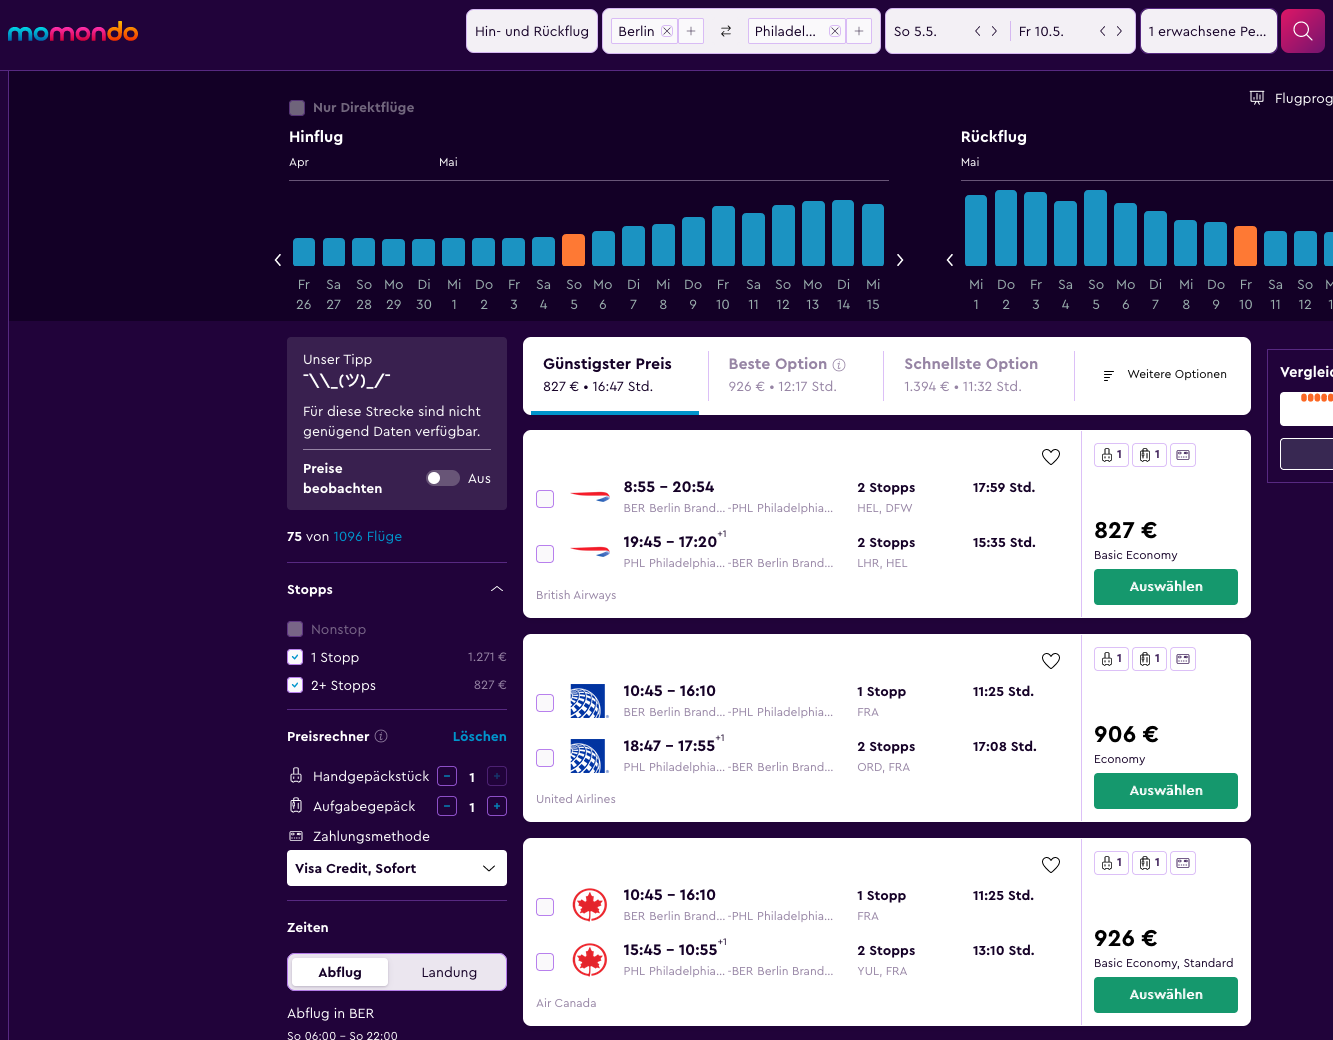
\includegraphics[width=0.9\textwidth]{./graphs/ccgrid2024.png}}
%     \caption{
%         Vergleichsangebote für die zeitgemäße An- und Abreise zur IEEE/ACM CCGrid 2024 vom 6.~bis 9.~Mai 2024 in Philadelphia, PA, USA.
%         Zuletzt abgerufen am 16.~Oktober 2023.
%     }
% \end{figure}

% \clearpage
\subsubsection{An-/Abreise IEEE IC2E 2024}
\label{sec:anhang:reisen:ic2e}

\begin{figure}[!h]
    \centering
    \fbox{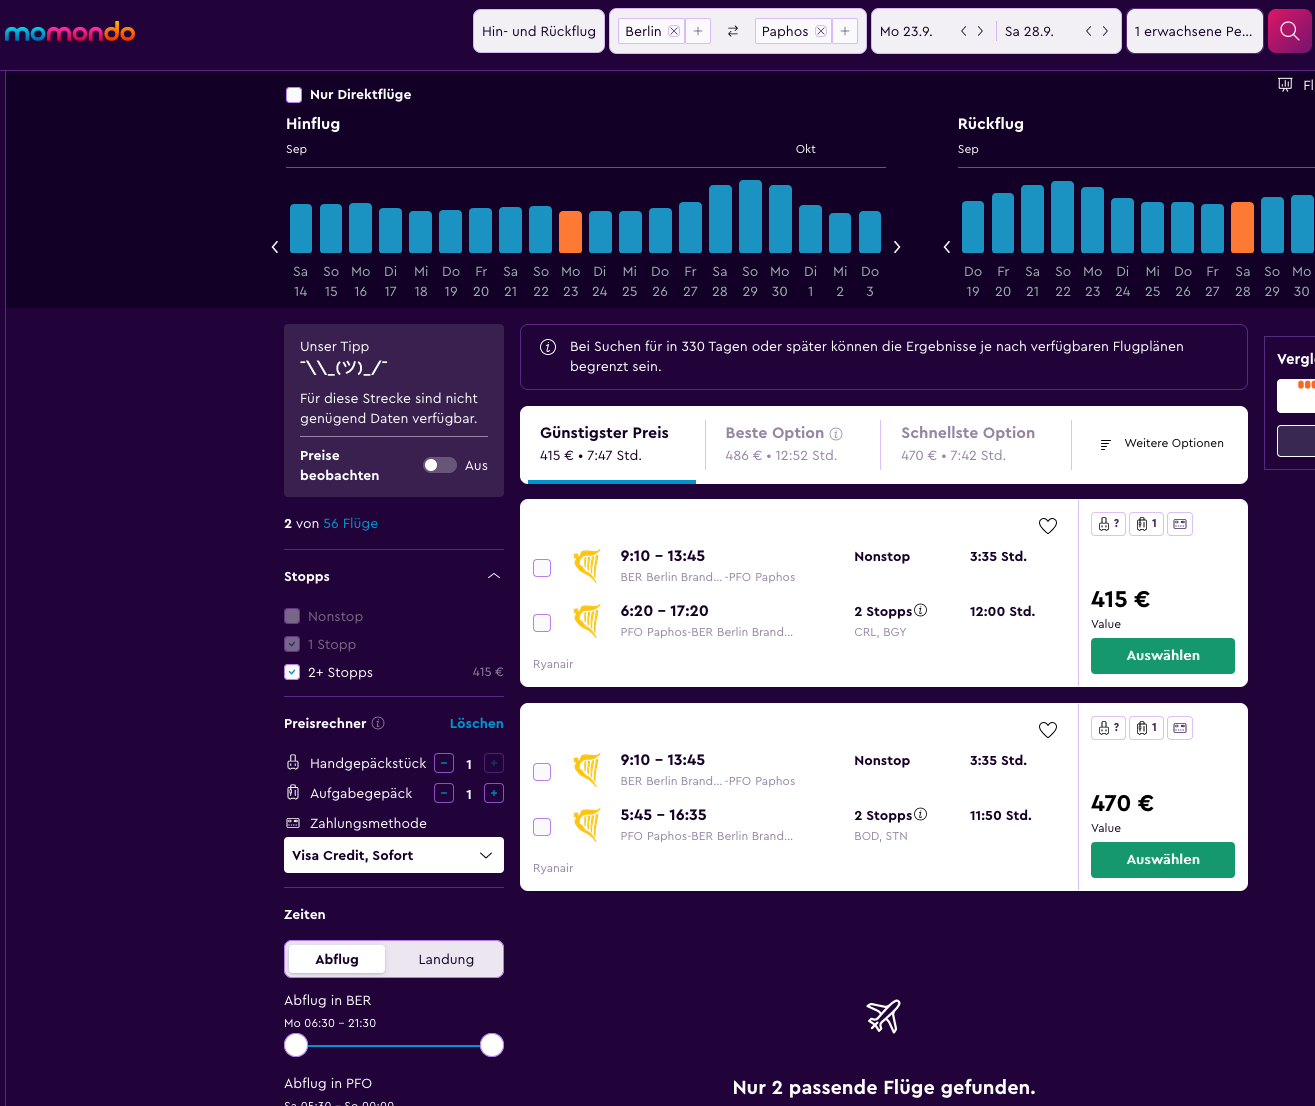
\includegraphics[width=0.9\textwidth]{./graphs/ic2e2024.png}}
    \caption{
        Vergleichsangebote für die zeitgemäße An- und Abreise zur IEEE IC2E 2024 vom 24.~bis 27.~September 2024 in Paphos, Zypern.
        Zuletzt abgerufen am 16.~Oktober 2023.
    }
\end{figure}

\clearpage
\subsubsection{An-/Abreise ACM/IFIP Middleware 2024}
\label{sec:anhang:reisen:middleware}

\begin{figure}[!h]
    \centering
    \fbox{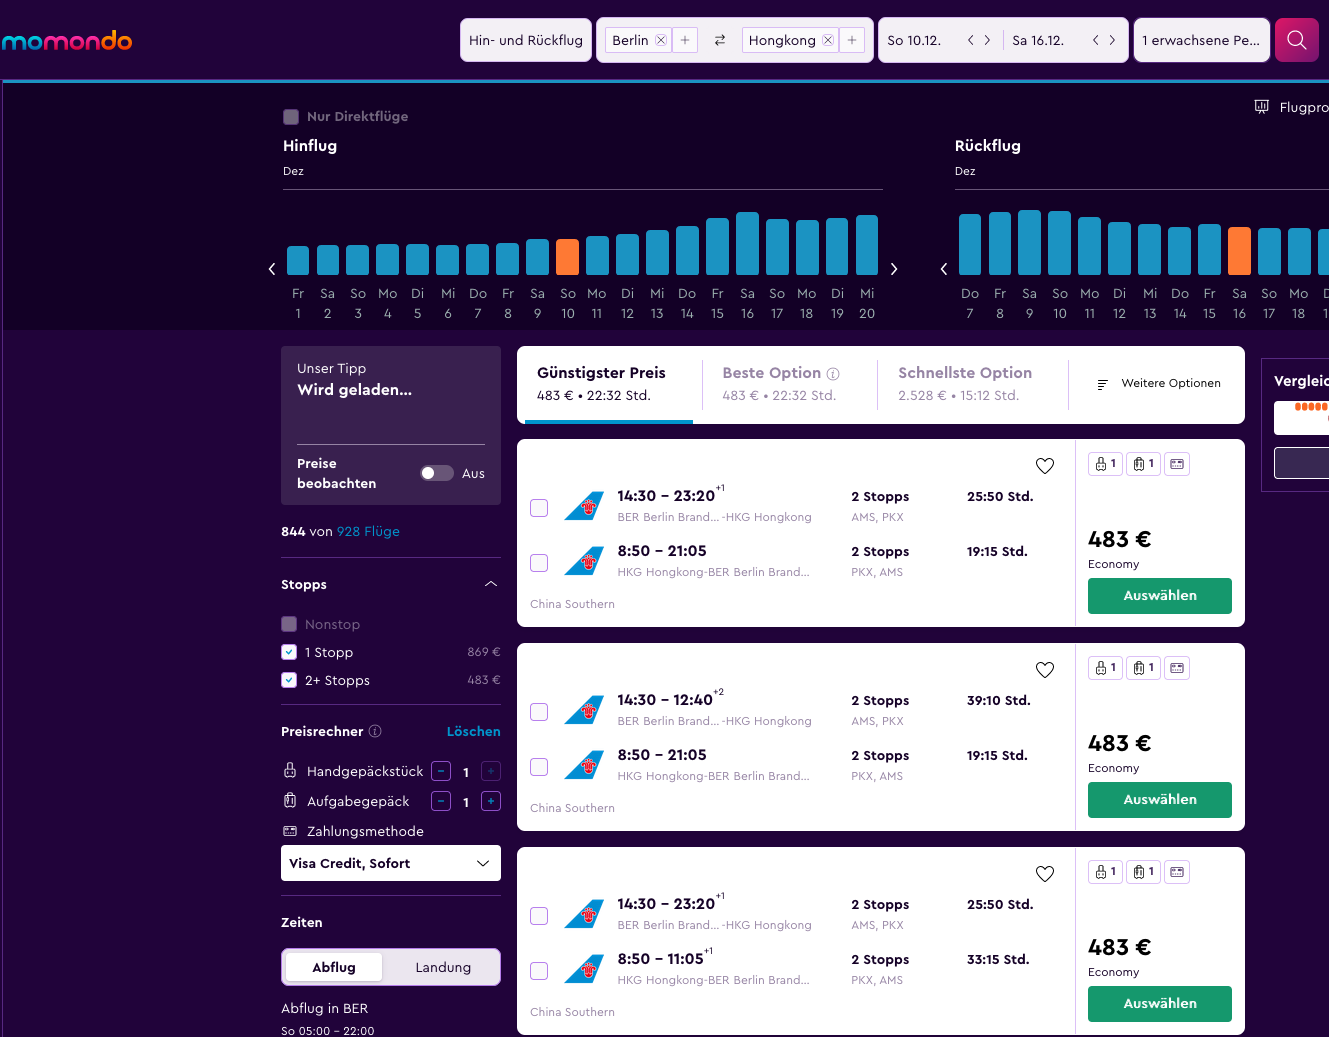
\includegraphics[width=0.9\textwidth]{./graphs/middleware2024neu.png}}
    \caption{
        Vergleichsangebote für die zeitgemäße An- und Abreise zur ACM/IFIP Middleware 2024 vom 11.~bis 15.~Dezember 2024 in Hongkong, SAR, China.
        Da die Reisedaten mehr als ein Jahr in der Zukunft liegen, sind noch keine Vergleichsangebote möglich.
        Es wird daher ein Vergleichsangebot für eine zeitgemäße Anreise für einen fiktiven Aufenthalt in Hongkong, SAR, China vom 11.~bis 15.~Dezember 2023 präsentiert.
        Zuletzt abgerufen am 09.~November 2023.
    }
\end{figure}

% \clearpage
% \subsubsection{An-/Abreise ACM EdgeSys 2024}
% \label{sec:anhang:reisen:edgesys}

% \begin{figure}[!h]
%     \centering
%     \fbox{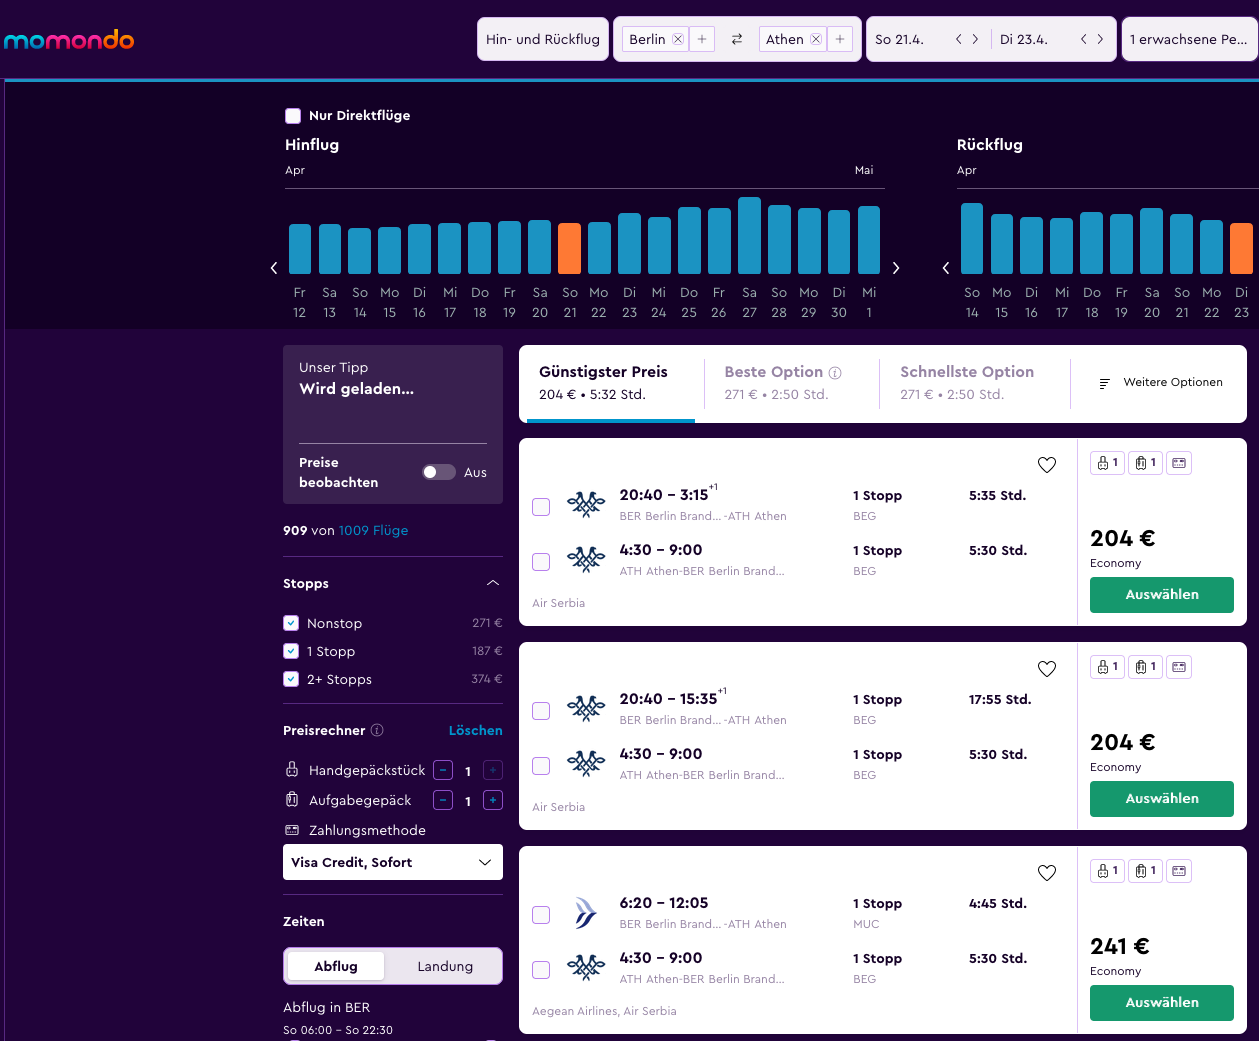
\includegraphics[width=0.9\textwidth]{./graphs/edgesys2024.png}}
%     \caption{
%         Vergleichsangebote für die zeitgemäße An- und Abreise zur /ACM EdgeSys 2024 am 22.~April 2024 in Athen, Griechenland.
%         Zuletzt abgerufen am 12.~Oktober 2023.
%     }
% \end{figure}

% \clearpage
% \subsubsection{An-/Abreise ACM LEO-NET 2024}
% \label{sec:anhang:reisen:leonet}

% \begin{figure}[!h]
%     \centering
%     \fbox{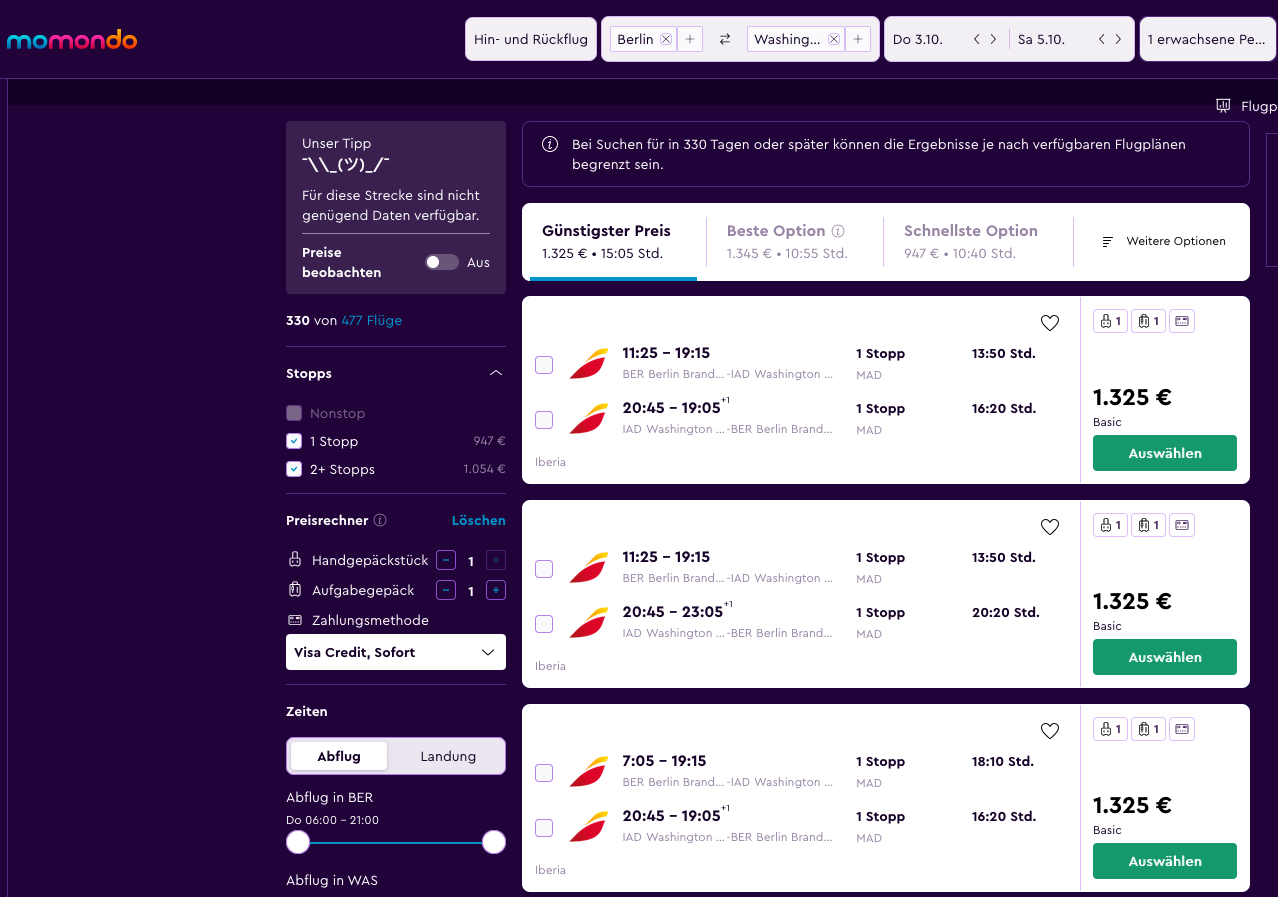
\includegraphics[width=0.9\textwidth]{./graphs/leonet2024.png}}
%     \caption{
%         Vergleichsangebote für die zeitgemäße An- und Abreise zur ACM LEO-NET 2024 am 4. Oktober 2024 in Washington, D.C., USA.
%         Zuletzt abgerufen am 12.~Oktober 2023.
%     }
% \end{figure}

% \clearpage
% \subsection{Angebot Cloud-Rechenkapazität}
% \label{sec:anhang:cloud}

% \begin{figure}[!h]
%     \centering
%     \fbox{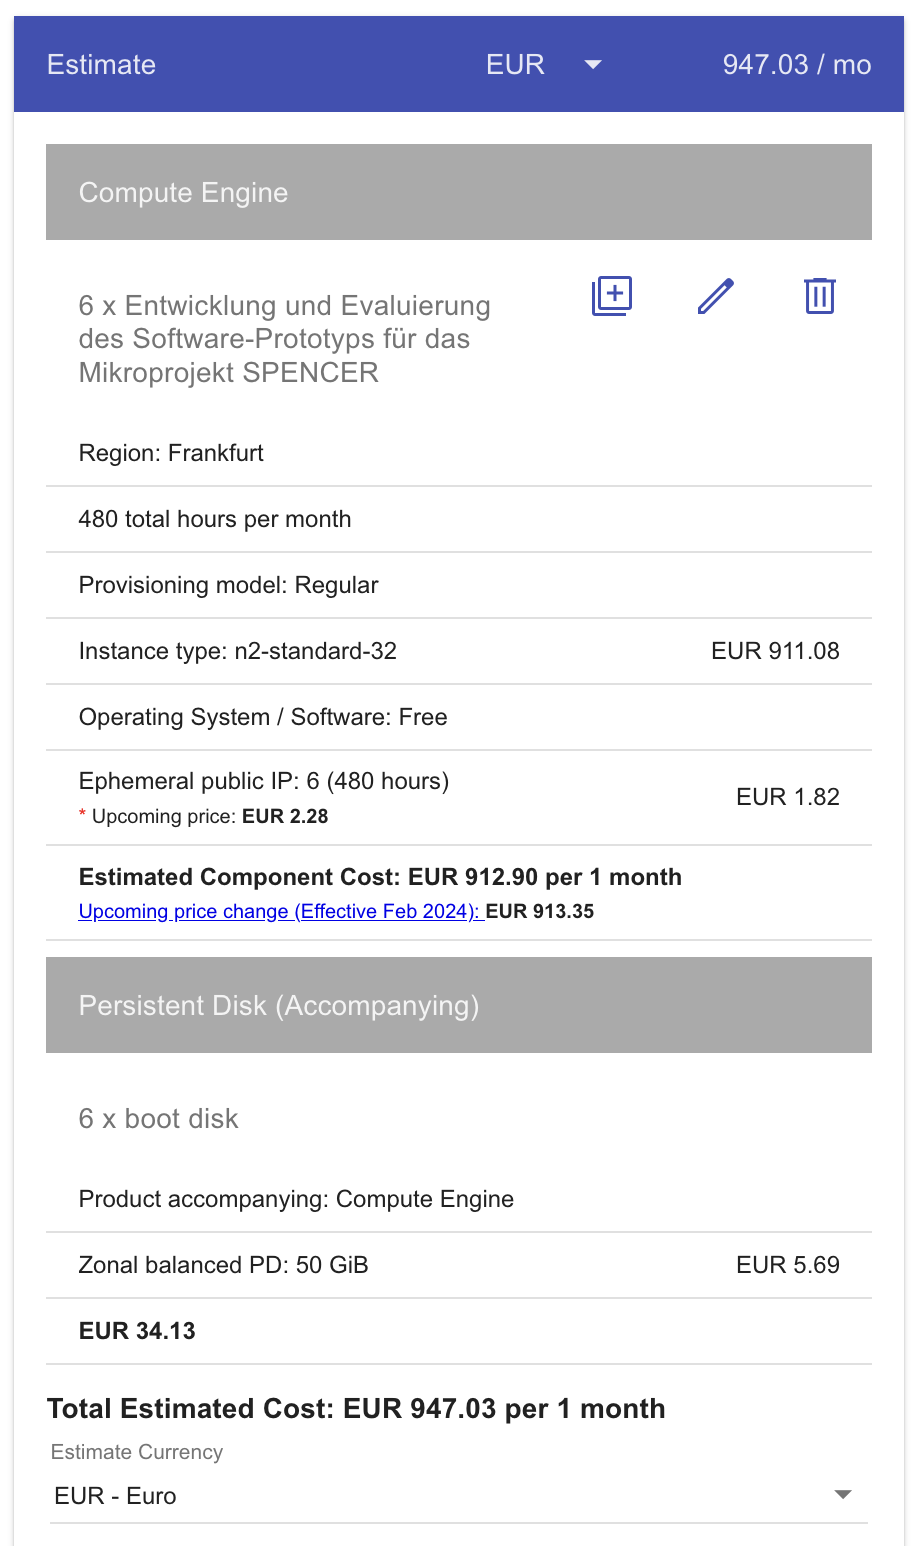
\includegraphics[width=8cm]{./graphs/gcloud.png}}
%     \caption{
%         Preiskalkulation für sechs Instanzen des Typs \texttt{n2-standard-32} in der Cloud-Region Frankfurt für einen Monat von 20 Arbeitstagen mit je vier Stunden Rechenkapazität.
%         Die angekündigte Preiserhöhung vor Projektstart ist zu beachten.
%         Digital einzusehen auf dem \href{https://cloud.google.com/products/calculator\#id=db406227-827f-458a-92e5-2d0f3c915a63}{Google Cloud Pricing Calculator} (Zuletzt abgerufen 15.~Oktober 2023).
%     }
% \end{figure}

% \clearpage
% \subsection{Angebote Demonstrator für Wissenschaftskommunikation}
% \label{sec:anhang:demonstrator}

% Der geplante Demonstrator für Wissenschaftskommunikation umfasst ein \emph{Samsung QB65B} 65-Zoll Public-Info-Display (\cref{sec:anhang:demonstrator:display}), einen \emph{MyWall HT21} Standfuß (\cref{sec:anhang:demonstrator:fuss}) und einen \emph{Lenovo ThinkCentre M60e Tiny 11LV0099GE} Slim-PC (\cref{sec:anhang:demonstrator:minipc}), für die hier jeweils drei Vergleichsangebote präsentiert werden.

% \subsubsection{Samsung QB65B 65-Zoll Public-Info-Display}
% \label{sec:anhang:demonstrator:display}

% \begin{figure}[!h]
%     \centering
%     \begin{subfigure}{1\linewidth}
%         \centering
%         \fbox{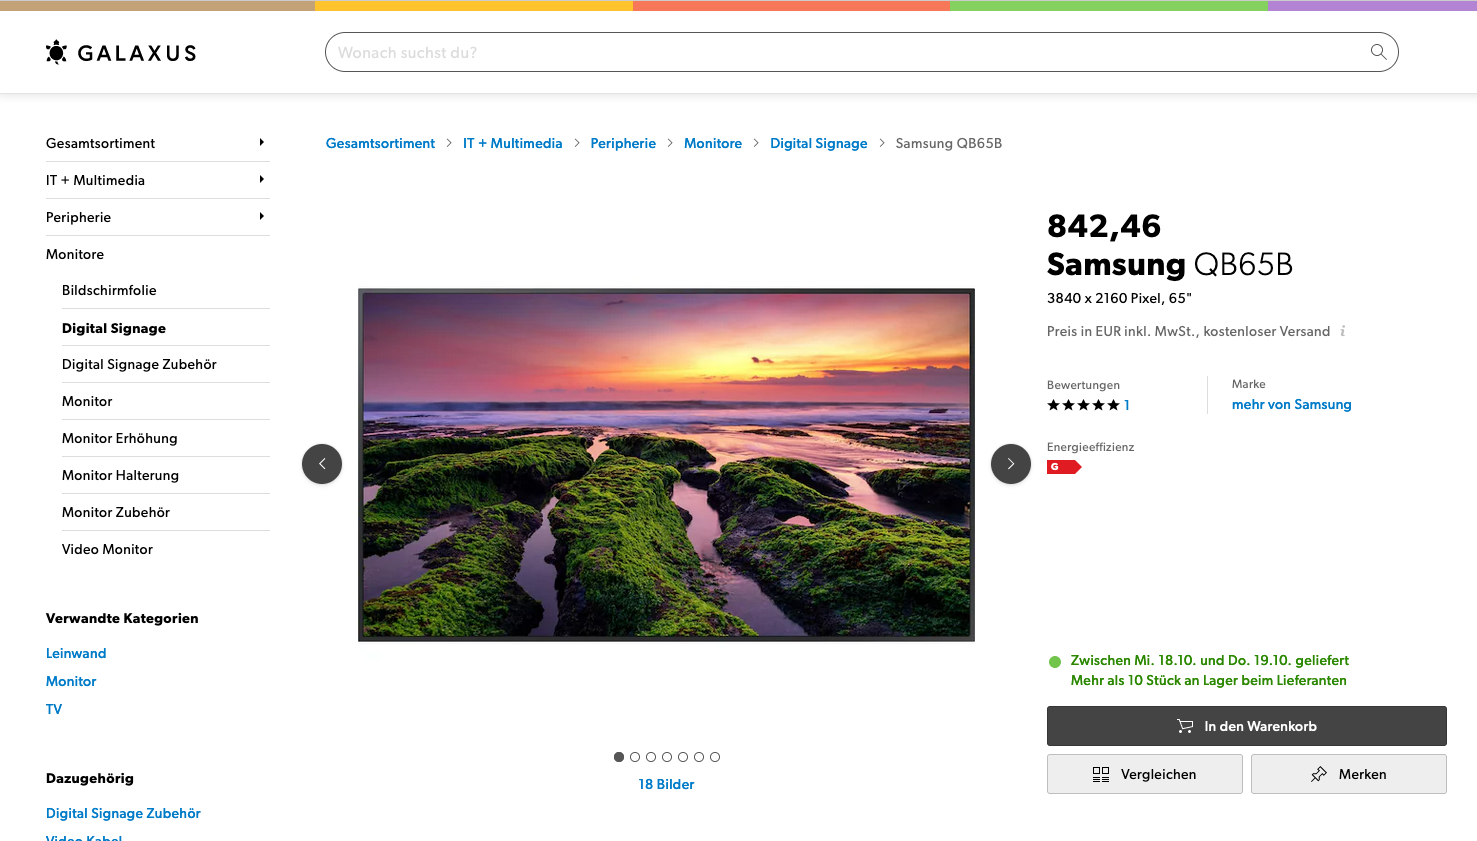
\includegraphics[width=0.5\linewidth]{./graphs/qb65b-galaxus.png}}
%         \caption{
%             Galaxus Deutschland GmbH -- 842,46~€ -- \href{https://www.galaxus.de/de/s1/product/samsung-qb65b-3840-x-2160-pixel-65-digital-signage-18596607}{Angebot}.
%         }
%     \end{subfigure}%
%     \vfill
%     \begin{subfigure}{1\linewidth}
%         \centering
%         \fbox{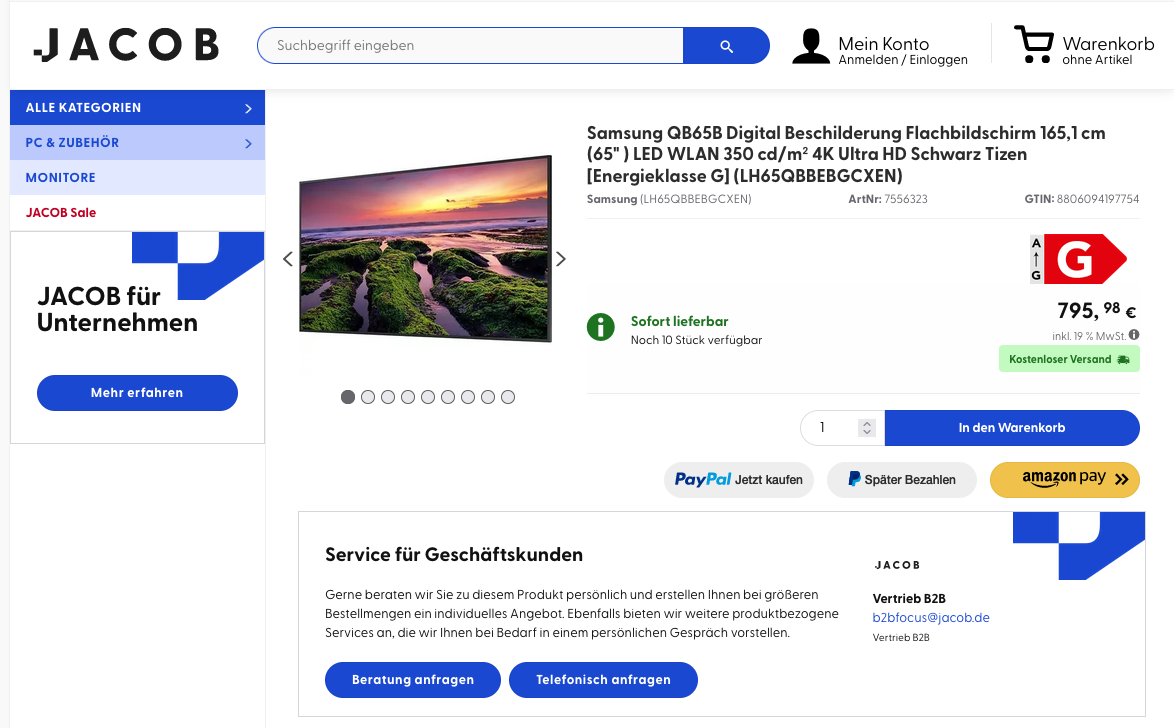
\includegraphics[width=0.5\linewidth]{./graphs/qb65b-jacob.png}}
%         \caption{
%             JACOB Elektronik GmbH -- 795,98~€ -- \href{https://direkt.jacob.de/produkte/samsung-qb65b-digital-lh65qbbebgcxen-artnr-7556323.html}{Angebot}.
%         }
%     \end{subfigure}%
%     \vfill
%     \begin{subfigure}{1\linewidth}
%         \centering
%         \fbox{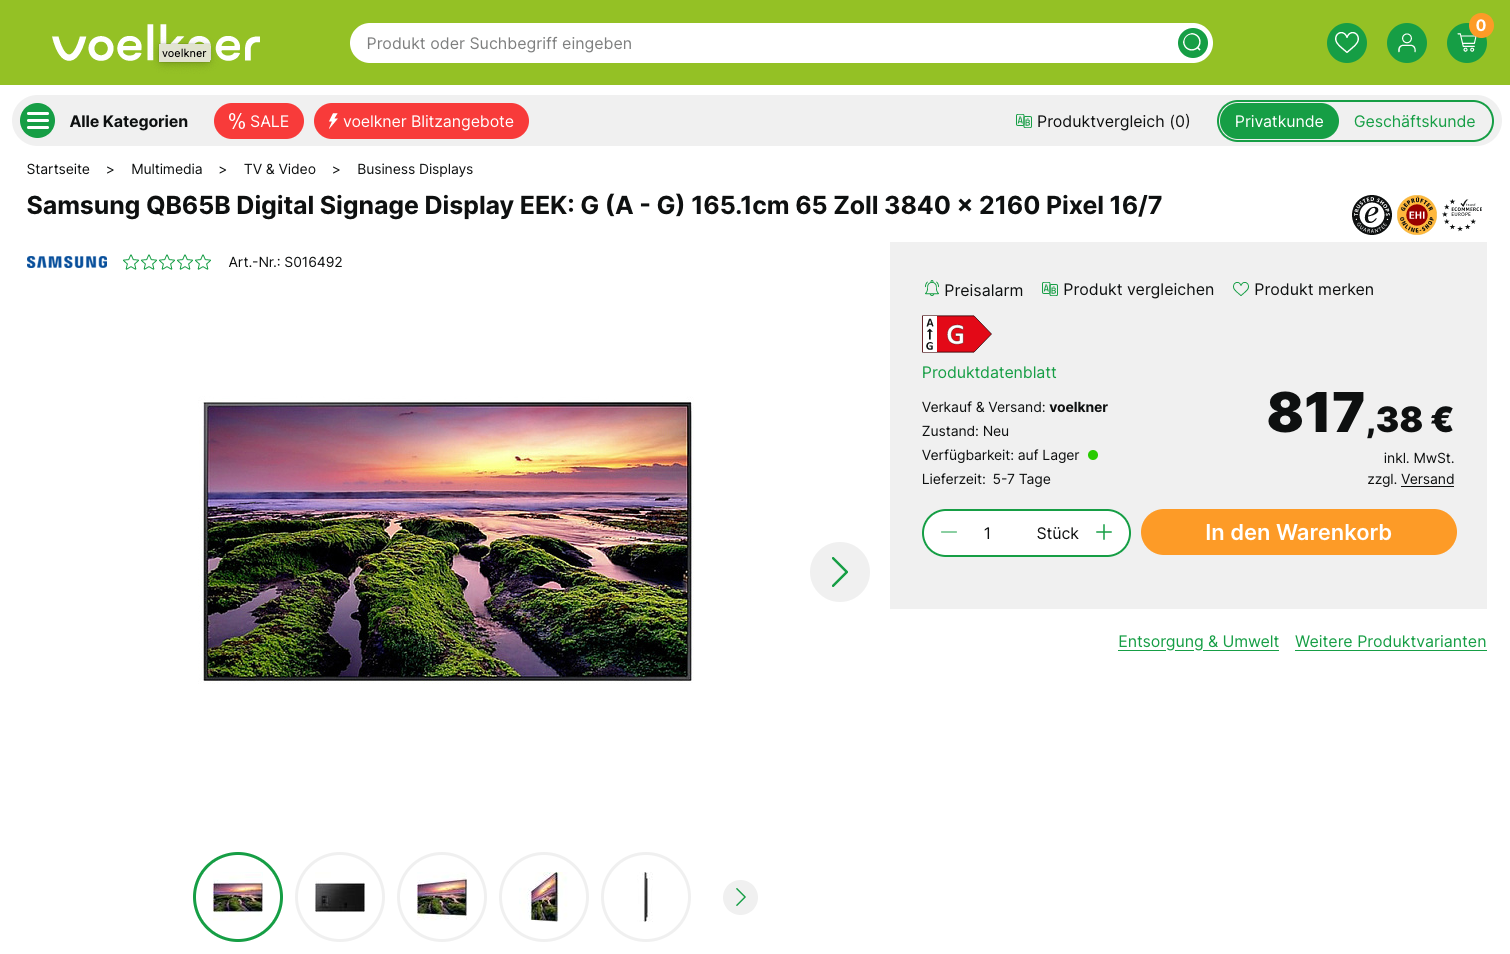
\includegraphics[width=0.5\linewidth]{./graphs/qb65b-voelkner.png}}
%         \caption{
%             RE-INvent Retail GmbH (voelkner) -- 817,38~€ -- \href{https://www.voelkner.de/products/5995608/Samsung-QB65B-Digital-Signage-Display-EEK-G-A-G-165.1cm-65-Zoll-3840-x-2160-Pixel-16-7.html}{Angebot}.
%         }
%     \end{subfigure}%
%     \caption{
%         Drei Vergleichsangebote für das \emph{Samsung QB65B} 65-Zoll Public-Info-Display.
%         Alle Preise inkl.~19\% MwSt.
%         Zuletzt abgerufen am 16.~Oktober 2023.
%     }
% \end{figure}

% \clearpage
% \subsubsection{MyWall HT21 Standfuß}
% \label{sec:anhang:demonstrator:fuss}

% \begin{figure}[!h]
%     \centering
%     \begin{subfigure}{1\linewidth}
%         \centering
%         \fbox{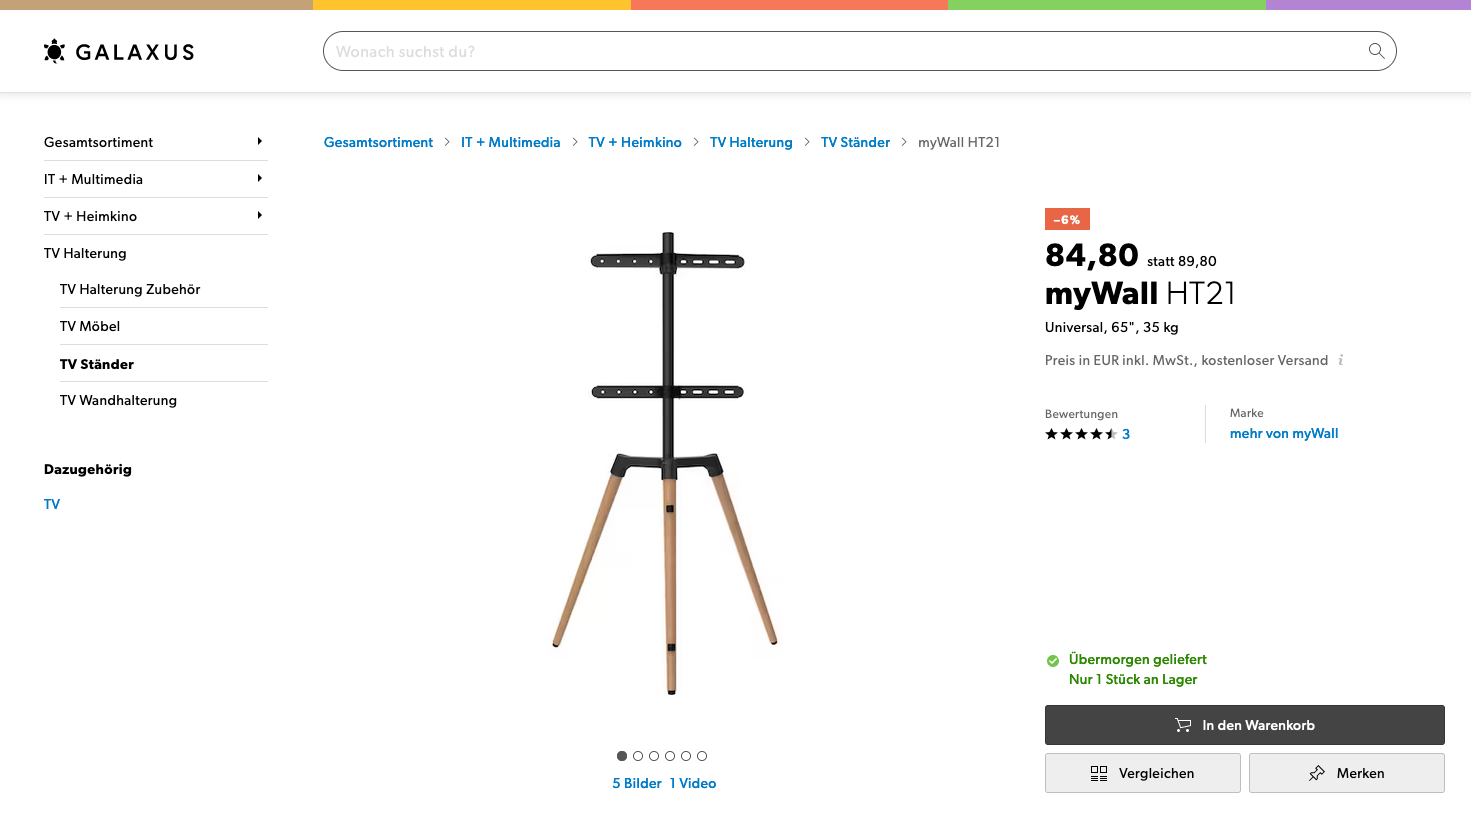
\includegraphics[width=0.6\linewidth]{./graphs/mywall-galaxus.png}}
%         \caption{
%             Galaxus Deutschland GmbH -- 84,80~€ -- \href{https://www.galaxus.de/de/s1/product/samsung-qb65b-3840-x-2160-pixel-65-digital-signage-18596607}{Angebot}.
%         }
%     \end{subfigure}%
%     \vfill
%     \begin{subfigure}{1\linewidth}
%         \centering
%         \fbox{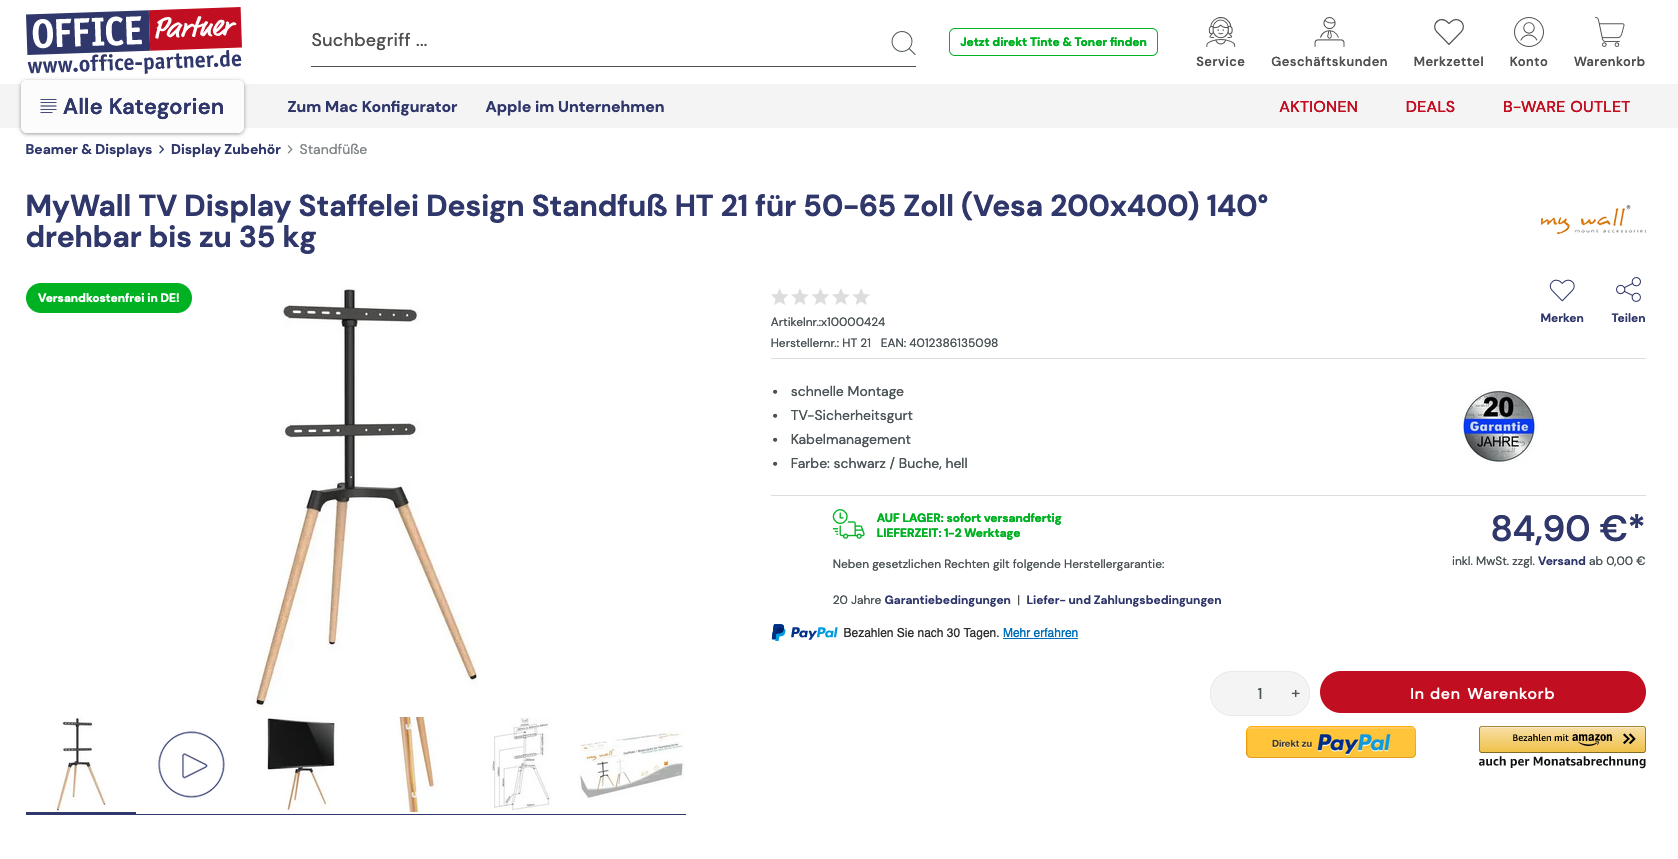
\includegraphics[width=0.6\linewidth]{./graphs/mywall-officepartner.png}}
%         \caption{
%             Office Partner GmbH -- 84,90~€ -- \href{https://www.office-partner.de/mywall-tv-display-staffelei-design-standfuss-ht21-x10000424}{Angebot}.
%         }
%     \end{subfigure}%
%     \vfill
%     \begin{subfigure}{1\linewidth}
%         \centering
%         \fbox{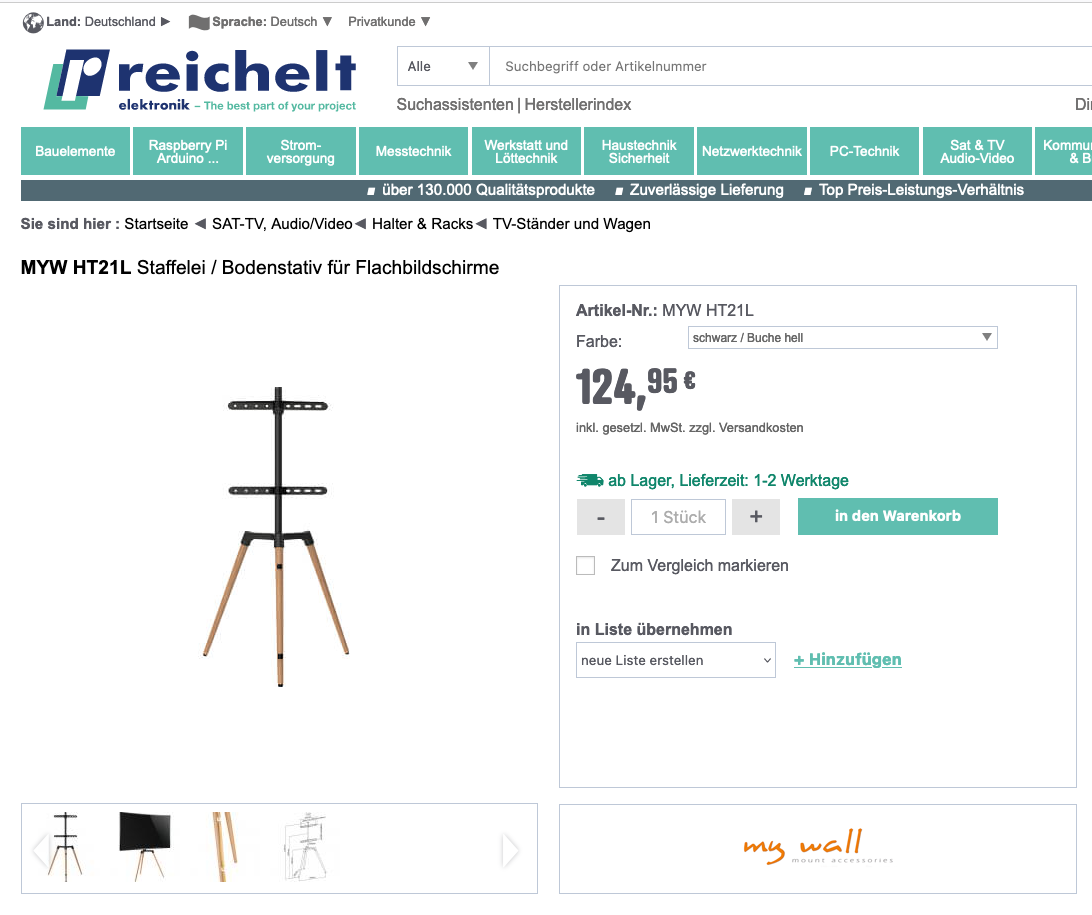
\includegraphics[width=0.6\linewidth]{./graphs/mywall-reichelt.png}}
%         \caption{
%             reichelt elektronik GmbH -- 124,95~€ -- \href{https://www.reichelt.de/staffelei-bodenstativ-fuer-flachbildschirme-myw-ht21l-p289195.html}{Angebot}.
%         }
%     \end{subfigure}%
%     \caption{
%         Drei Vergleichsangebote für den \emph{MyWall HT21} Standfuß.
%         Alle Preise inkl.~19\% MwSt.
%         Zuletzt abgerufen am 16.~Oktober 2023.
%     }
% \end{figure}

% \clearpage
% \subsubsection{Lenovo ThinkCentre M60e Tiny 11LV0099GE Slim-PC}
% \label{sec:anhang:demonstrator:minipc}

% \begin{figure}[!h]
%     \centering
%     \begin{subfigure}{1\linewidth}
%         \centering
%         \fbox{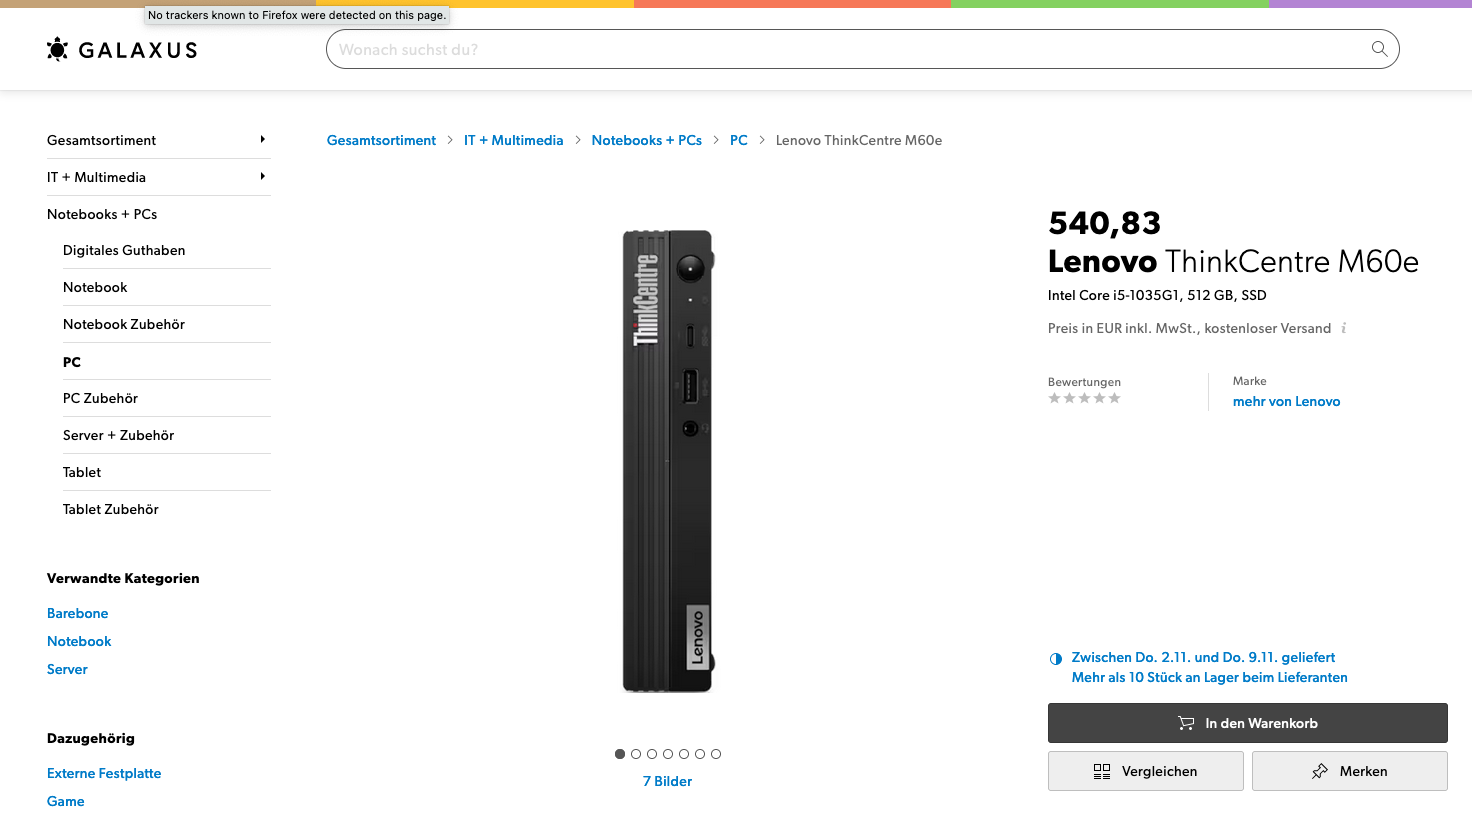
\includegraphics[width=0.6\linewidth]{./graphs/m60e-galaxus.png}}
%         \caption{
%             Galaxus Deutschland GmbH -- 540,83~€ -- \href{https://www.galaxus.de/de/s1/product/lenovo-thinkcentre-m60e-intel-core-i5-1035g1-512-gb-ssd-pc-24364370}{Angebot}.
%         }
%     \end{subfigure}%
%     \vfill
%     \begin{subfigure}{1\linewidth}
%         \centering
%         \fbox{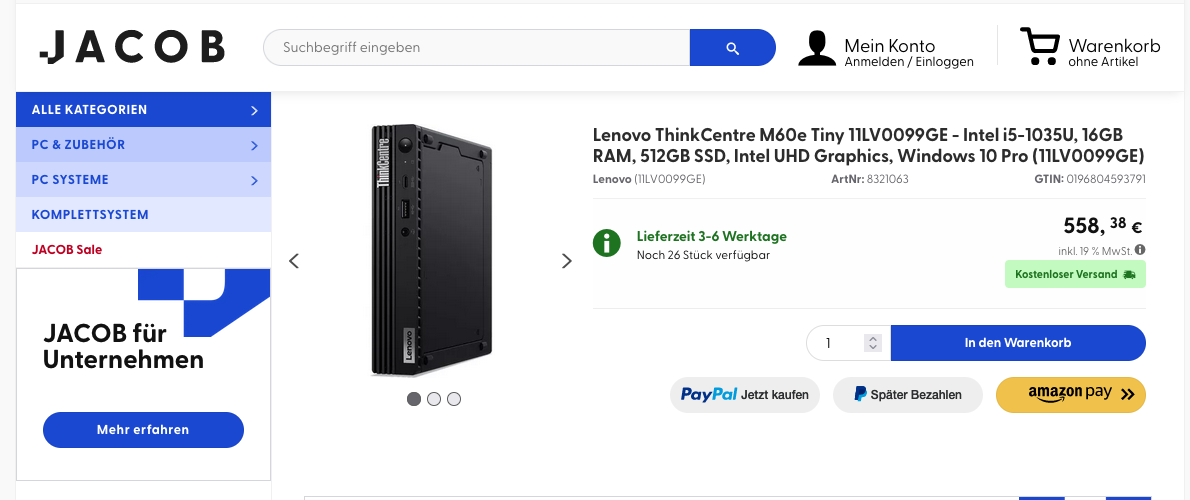
\includegraphics[width=0.6\linewidth]{./graphs/m60e-jacob.png}}
%         \caption{
%             JACOB Elektronik GmbH -- 558,38~€ -- \href{https://direkt.jacob.de/produkte/lenovo-thinkcentre-m60e-11lv0099ge-artnr-8321063.html}{Angebot}.
%         }
%     \end{subfigure}%
%     \vfill
%     \begin{subfigure}{1\linewidth}
%         \centering
%         \fbox{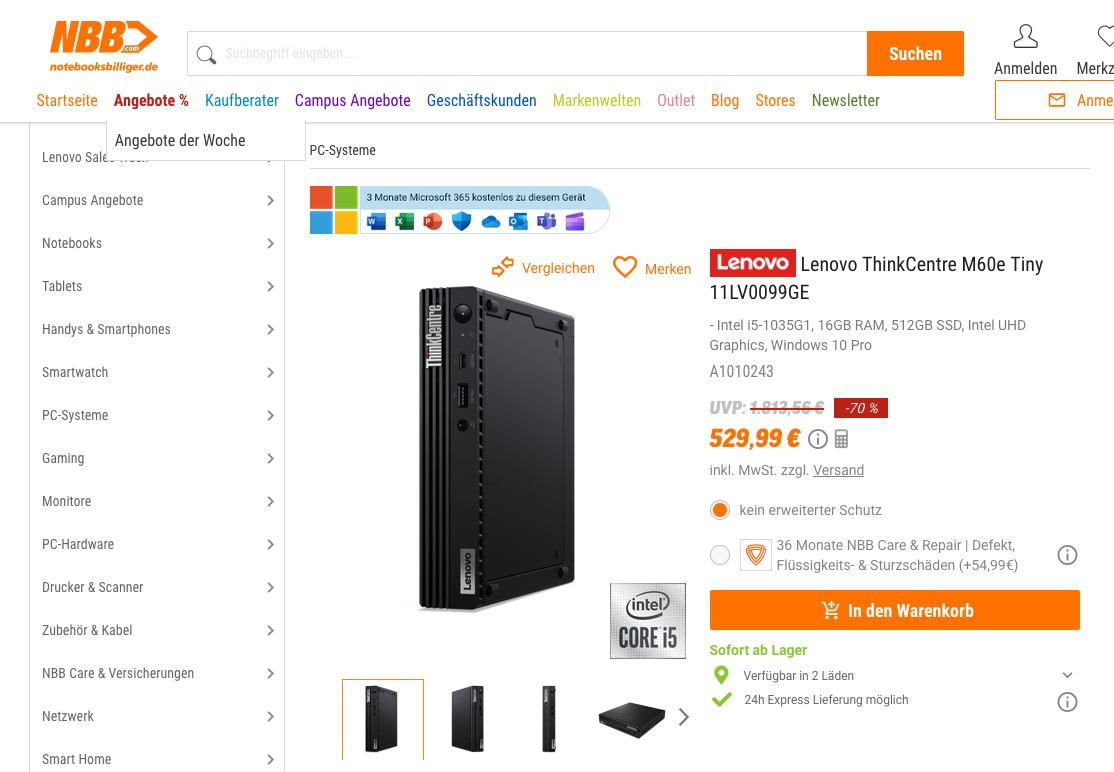
\includegraphics[width=0.6\linewidth]{./graphs/m60e-nbb.png}}
%         \caption{
%             notebooksbilliger.de AG -- 529,99~€ -- \href{https://www.notebooksbilliger.de/lenovo+thinkcentre+m60e+tiny+11lv0099ge+796837}{Angebot}.
%         }
%     \end{subfigure}%
%     \caption{
%         Drei Vergleichsangebote für einen \emph{Lenovo ThinkCentre M60e Tiny 11LV0099GE} Slim-PC.
%         Alle Preise inkl.~19\% MwSt.
%         Zuletzt abgerufen am 16.~Oktober 2023.
%     }
% \end{figure}


\end{document}

